%definira klasu dokumenta 
\documentclass[12pt]{report} 

%prostor izmedu naredbi \documentclass i \begin{document} se zove uvod. U njemu se nalaze naredbe koje se odnose na cijeli dokument

%osnovni LaTex ne može riješiti sve probleme, pa se koriste različiti paketi koji olakšavaju izradu željenog dokumenta
\usepackage[croatian]{babel} 
\usepackage{amssymb}
\usepackage{amsmath}
\usepackage{txfonts}
\usepackage{mathdots}
\usepackage{titlesec}
\usepackage{array}
\usepackage{lastpage}
\usepackage{etoolbox}
\usepackage{tabularray}
\usepackage{color, colortbl}
\usepackage{adjustbox}
\usepackage{geometry}
\usepackage[classicReIm]{kpfonts}
\usepackage{hyperref}
\usepackage{fancyhdr}

\usepackage{float}
\usepackage{setspace}
\restylefloat{table}


\patchcmd{\chapter}{\thispagestyle{plain}}{\thispagestyle{fancy}}{}{} %redefiniranje stila stranice u paketu fancyhdr

%oblik naslova poglavlja
\titleformat{\chapter}{\normalfont\huge\bfseries}{\thechapter.}{20pt}{\Huge}
\titlespacing{\chapter}{0pt}{0pt}{40pt}


\linespread{1.3} %razmak između redaka

\geometry{a4paper, left=1in, top=1in,}  %oblik stranice

\hypersetup{ colorlinks, citecolor=black, filecolor=black, linkcolor=black,	urlcolor=black }   %izgled poveznice


%prored smanjen između redaka u nabrajanjima i popisima
\newenvironment{packed_enum}{
	\begin{enumerate}
		\setlength{\itemsep}{0pt}
		\setlength{\parskip}{0pt}
		\setlength{\parsep}{0pt}
	}{\end{enumerate}}

\newenvironment{packed_item}{
	\begin{itemize}
		\setlength{\itemsep}{0pt}
		\setlength{\parskip}{0pt}
		\setlength{\parsep}{0pt}
	}{\end{itemize}}




%boja za privatni i udaljeni kljuc u tablicama
\definecolor{LightBlue}{rgb}{0.9,0.9,1}
\definecolor{LightGreen}{rgb}{0.9,1,0.9}

%Promjena teksta za dugačke tablice
\DefTblrTemplate{contfoot-text}{normal}{Nastavljeno na idućoj stranici}
\SetTblrTemplate{contfoot-text}{normal}
\DefTblrTemplate{conthead-text}{normal}{(Nastavljeno)}
\SetTblrTemplate{conthead-text}{normal}
\DefTblrTemplate{middlehead,lasthead}{normal}{Nastavljeno od prethodne stranice}
\SetTblrTemplate{middlehead,lasthead}{normal}

%podesavanje zaglavlja i podnožja

\pagestyle{fancy}
\lhead{Programsko inženjerstvo}
\rhead{$<$Projektni zadatak$>$}
\lfoot{$<$Naziv grupe$>$}
\cfoot{stranica \thepage/\pageref{LastPage}}
\rfoot{\today}
\renewcommand{\headrulewidth}{0.2pt}
\renewcommand{\footrulewidth}{0.2pt}


\begin{document} 
	
	
	
	\begin{titlepage}
		\begin{center}
			\vspace*{\stretch{1.0}} %u kombinaciji s ostalim \vspace naredbama definira razmak između redaka teksta
			\LARGE Programsko inženjerstvo\\
			\large Ak. god. 2020./2021.\\
			
			\vspace*{\stretch{3.0}}
			
			\huge $<$Naziv projekta$>$\\
			\Large Dokumentacija, Rev. \textit{$<$1 ili 2$>$}\\
			
			\vspace*{\stretch{12.0}}
			\normalsize
			Grupa: \textit{$<$Naziv grupe$>$}\\
			Voditelj: \textit{$<$Ime i prezime voditelja$>$}\\
			
			
			\vspace*{\stretch{1.0}}
			Datum predaje: \textit{$<$dan$>$. $<$mjesec$>$. $<$godina$>$.}\\
	
			\vspace*{\stretch{4.0}}
			
			Nastavnik: \textit{$<$Ime i prezime nastavnika zaduženog za vašu grupu$>$}\\
		
		\end{center}

	
	\end{titlepage}

	
	\tableofcontents


	\chapter{Dnevnik promjena dokumentacije}
		
		\textbf{\textit{Kontinuirano osvježavanje}}\\
				
		
		\begin{longtblr}[
				label=none
			]{
				width = \textwidth, 
				colspec={|X[2]|X[13]|X[3]|X[3]|}, 
				rowhead = 1
			}
			\hline
			\textbf{Rev.}	& \textbf{Opis promjene/dodatka} & \textbf{Autori} & \textbf{Datum}\\[3pt] \hline
			0.1 & Napravljena inicijalna skica toka i obrazaca upotrebe. & svi & 23.10.2023. 		\\[3pt] \hline 
			0.2	& Dodani funkcionalni zahtjevi.\newline Dodani obrasci uporabe. & Tea, Nikola, Ivan & 05.11.2023. 	\\[3pt] \hline
            0.2.1 & Revizija funkcionalnih zahtjeva i obrazaca uporabe. & Karlo & 07.11.2023. 	\\[3pt] \hline
			0.3 & Dodan \textit{Use Case} dijagram i četiri sekvencijska dijagrama. \newline Dodatna revizija obrazaca uporabe. & Niko, Ivan & 09.11.2023. \\[3pt] \hline 
			0.4 & Dodan opis baze podataka. & Tea & 12.11.2023. \\[3pt] \hline 
            0.5 & Dodan opis arhitekture. & Tea, Karlo & 14.11.2023. \\[3pt] \hline 
			0.6 & Napisan \textit{Opis projektnog zadatka}, \textit{Dodatak}, \textit{Nefunkcionalni zahtjevi} i \textit{Dnevnik promjena} & Karlo & 14.11.2023. \\[3pt] \hline 
			\textbf{1.0} & Verzija samo s bitnim dijelovima za 1. ciklus & svi & 17.11.2023. \\[3pt] \hline 
			1.1 & Dodan dijagram stanja & Tea & 06.01.2024 \\[3pt] \hline 
			1.2 & Dodan dijagram aktivnosti & Nikola & 07.01.2024. \\[3pt] \hline 
			1.3 & Dodan dijagram komponenti & Ivan & 09.01.2024. \\[3pt] \hline 
			1.4 & Napisan zaključak & Tea & 14.01.2024. \\[3pt] \hline 
			1.5 & Dodan dijagram razmještaja & Ivan & 15.01.2024. \\[3pt] \hline 
			1.6 & Napisane upute za puštanje u pogon & Tea & 16.01.2024. \\[3pt] \hline 
			1.7 & Revizija dijagrama aktivnosti, tablice aktivnosti, dnevnika promjena 
			dokumentacije, dnevnika sastanaka, zaključka, uputa za pogon 
			dodano ispitivanje programskog rješenja, prikaz aktivnosti grupe
			&  Ivan, Tea, Nikola & 19.1.2024.\\[3pt] \hline
			\textbf{2.0} & Konačni tekst predloška dokumentacije  & svi & 19.01.2024. \\[3pt] \hline 
			
		\end{longtblr}
	
	
	\chapter{Opis projektnog zadatka}
		
		\textbf{\textit{dio 1. revizije}}\\

        \section*{Uvod}

        Jedan od ključnih izazova s kojima se suočavamo u \textit{suvremenom zdravstvu} jest \textbf{neefikasnost sustava dodjele termina} i upravljanja medicinskim procesima. Područje u kojem je to zbog svoje bliskosti s "običnim" čovjekom posebno evidentno jesu \textbf{sustavi rehabilitacije}. Njih karakterizira kompleksnost potreba pacijenata, raznolikost terapijskih pristupa i ograničeni resursi, posebno izraženi u kontekstu hrvatskog zdravstva. Dosadašnji \textbf{manualni procesi} evidencije i upravljanja terminima često dovode do neoptimalnog iskorištavanja već oskudnih resursa.
        
        \subsection*{\textbf{\large Potreba za inovacijom}}
        Postoji očita potreba za razvojem \textit{novog sustava} koji će omogućiti bolje upravljanje rehabilitacijskim procesima, povećati efikasnost i znatno unaprijediti iskustvo i zadovoljstvo pacijenata.
        
        \subsection*{\textbf{\large Transformacija procesa}}
        Projekt je započeo s vizijom transformacije postojećih manualnih procesa u \textbf{automatizirani, digitalizirani sustav}. Cilj nam je bio kreiranje platforme koja optimizira raspodjelu termina, \textbf{povećava efikasnost} i pruža transparentnost u praćenju i upravljanju procesima rehabilitacije.
        
        \subsection*{\textbf{\large Inkluzivnost i dostupnost}}
        Fokus projekta bio je na razvoju \textit{inkluzivnog} servisa dostupnog za široku populaciju. Zbog toga je potrebno omogućiti jednostavno korištenje platforme za sve članove društva, uključujući pacijente i djelatnike.
        
        \subsection*{\textbf{\large Razvoj web aplikacije}}
        Ključni dio projekta uključuje razvoj web aplikacije koja bolesnicima omogućava prijavu na rehabilitaciju, odabir terapije i termine te praćenje njihovog napretka. Djelatnicima zdravstvene ustanove pruža se niz alata za efikasno upravljanje terminima i bilježenje napretka pacijenata, dok se administratorima omogućava upravljanje korisničkim računima i resursima.


        \section*{Funkcionalnost aplikacije}

        Aplikacija je zamišljena tako da omogućuje bolesnicima prijavu na rehabilitaciju i praćenje napretka te sljedećih termina u stvarnom vremenu. S druge strane, djelatnici imaju interaktivan raspored kojem mogu pristupiti u bilo kojem trenutku, dok administratori nadziru sve termine i rasporede kako bi bili sigurni da je čitav proces optimiziran. \\
        
        U našoj aplikaciji, interakcija između glavnih dionika - bolesnika, djelatnika zdravstvene ustanove i administratora sustava - ključna je za njezin uspješan rad. Svaki od ovih dionika ima specifične uloge i funkcionalne zahtjeve.
        
        \subsection*{Administratori sustava}
        \begin{itemize}
            \item \textbf{Upravljanje korisnicima:} Administratori imaju ključnu ulogu u upravljanju korisničkim računima, kako za djelatnike, tako i za bolesnike. Oni mogu prihvatiti ili odbiti registracije te uređivati ili brisati postojeće račune.
            
            \item \textbf{Nadzor termina:} Odgovorni su za pregled i potvrdu prijava bolesnika za rehabilitaciju te mogu otkazati ili pomaknuti zakazane termine.
        
            \item \textbf{Pristup i analiza podataka:} Administratori imaju pristup cjelokupnoj bazi podataka, omogućavajući im nadzor i analizu svih aspekata rehabilitacijskog procesa.
        \end{itemize}
        
        \subsection*{Djelatnici zdravstvene ustanove}
        \begin{itemize}
            \item \textbf{Bilježenje napretka:} Djelatnici mogu bilježiti napredak bolesnika tijekom rehabilitacijskih sesija, što je ključno za praćenje i prilagodbu terapijskih pristupa.
        
            \item \textbf{Upravljanje rasporedom:} Imaju mogućnost pregleda i upravljanja vlastitim rasporedom sesija, kao i pristup podacima o bolesnicima.
        
            \item \textbf{Komunikacija s bolesnicima:} Mogućnost otkazivanja sesija pod određenim uvjetima omogućava djelatnicima fleksibilnost u upravljanju izvanrednim situacijama.
        \end{itemize}
        
        \subsection*{bolesnici}
        \begin{itemize}
            \item \textbf{Proces registracije i prijave:} Bolesnici se mogu registrirati u sustav, prijaviti se i pristupiti svojim profilima za praćenje rehabilitacije.
        
            \item \textbf{Praktične mogućnosti:} Mogu se prijaviti na rehabilitaciju, odabrati terapiju, termine dolaska (koji prate pravila specifične terapije) te pratiti svoje termine i povijest terapija. U iznimnim situacijama mogu pomaknuti termin. 
        
            \item \textbf{Pristup informacijama:} Imaju pristup svom kalendaru s terminima terapije što im omogućava bolje planiranje i organizaciju.
        \end{itemize}
        
        \subsection*{Baza podataka}
        \begin{itemize}
            \item \textbf{Središnje skladište podataka:} Sve informacije o bolesnicima, djelatnicima i rehabilitacijskim sesijama pohranjuju se u bazi podataka čime se osigurava integracija i efikasnost sustava.
        \end{itemize}
        
        \eject
        
        

        \section*{Poslovni model}
        
        \subsection*{B2B model i implementacija u bolničkom sustavu}
        \begin{itemize}
            \item \textbf{Orijentacija na bolnički sustav:} Naša aplikacija je primarno namijenjena upotrebi unutar \textit{bolničkog sustava}, što je usko povezano s B2B (business-to-business) modelom. Ovaj pristup podrazumijeva da naša aplikacija nije direktno namijenjena pojedinačnim korisnicima, već bolnicama i poliklinikama kao korporativnim klijentima.
            
            \item \textbf{Razina implementacije:} Uspješna implementacija aplikacije zahtijeva široku adaptaciju, idealno na nacionalnoj razini ili barem unutar privatnih poliklinika za rehabilitaciju. Takav pristup omogućuje efikasniju koordinaciju i standardizaciju procesa rehabilitacije.
            
            \item \textbf{Značaj skalabilnosti:} Naš fokus je bio na razvoju aplikacije koja je fleksibilna i skalabilna, sposobna prilagoditi se različitim veličinama i vrstama zdravstvenih ustanova.
        \end{itemize}
        
        \subsection*{Ekspanzija i skalabilnost}
        \begin{itemize}
            \item \textbf{Faza početne implementacije:} Trenutno je aplikacija razvijena za upotrebu unutar jedne bolnice ili poliklinike za rehabilitaciju. Ovaj početni pristup omogućuje nam detaljno testiranje i optimizaciju funkcionalnosti aplikacije.
            
            \item \textbf{Strategije ekspanzije:} U razmatranju načina ekspanzije identificirali smo dva glavna pristupa:
                \begin{enumerate}
                    \item \textit{Individualizirani sustavi:} Razvijanje \textit{custom} verzije aplikacije za svaku bolnicu. Svaka ustanova imala bi svoju prilagođenu verziju aplikacije što bi moglo poslužiti kao dodatni faktor privlačnosti za klijente.
                    
                    \item \textit{Centralizirani sustav:} Stvaranje jedne velike centralizirane aplikacije. Ovaj pristup uključuje izbor institucije na početku korištenja aplikacije.
                \end{enumerate}
            
            \item \textbf{Potencijal za daljnju ekspanziju:} Oba pristupa imaju svoje prednosti i izazove te pružaju različite mogućnosti za daljnju ekspanziju i adaptaciju aplikacije, u skladu s potrebama tržišta i specifičnostima korisnika. Lako je moguće da bismo se odlučili za \textit{hibridni pristup} gdje bi svaka bolnica imala naizgled "svoju" aplikaciju "hostiranu" na \textit{custom} domeni, s vizualno prilagođenim korisničkim sučeljem (UI). Ovaj pristup kombinira prednosti individualiziranih i centraliziranih sustava omogućujući bolnicama da se osjećaju kao da imaju jedinstveno, prilagođeno rješenje dok se u stvarnosti koristi jedan centralizirani sustav.

            Pod "haubom", sve bi aplikacije bile zasnovane na istoj osnovnoj arhitekturi i dijelile isti skup funkcionalnosti. To bi omogućilo efikasnije održavanje i ažuriranje sustava dok bi korisnici imali dojam personaliziranog iskustva. Tehnički, ovakav pristup može se postići korištenjem \textit{proxy servera} ili sličnih tehnologija za usmjeravanje prometa na odgovarajuće instance aplikacije omogućujući tako svakoj bolnici da ima svoju unikatnu URL adresu i prilagođen UI. Ovaj hibridni model pruža fleksibilnost u pružanju usluga klijentima, dok istovremeno minimizira troškove i složenost održavanja više odvojenih instanci aplikacije.

            \end{itemize}
            
            \subsection*{Analiza konkurencije:} 
                Konkurenciju najbolje možemo podijeliti u dvije grupe: 
                \begin{itemize}
                    \item \textbf{Manualni sustavi:} Naša prva i najizazovnija konkurencija su postojeći manualni sustavi. Promjena navika i entuzijazam djelatnika za učenje nečega novog predstavljaju značajne prepreke.
                    \item \textbf{Digitalna rješenja:} Iako je teško pronaći konkretna B2B rješenja putem običnog pretraživanja, neka od rješenja koja smo identificirali uključuju:
                    \begin{itemize}
                        \item \textbf{MedBridge Go:} Radi se o aplikaciji koja je pretežno usmjerena odrađivanju vježbi koje je doktor propisao kod kuće. 
                        Također postoje posebni profili za liječnika i pacijenta, ali ovdje se ne delegira resursima odjela za fizikalnu terapiju te zbog toga nije direktna konkurencija. 
                        \begin{figure}[!h]
                            \centering
                            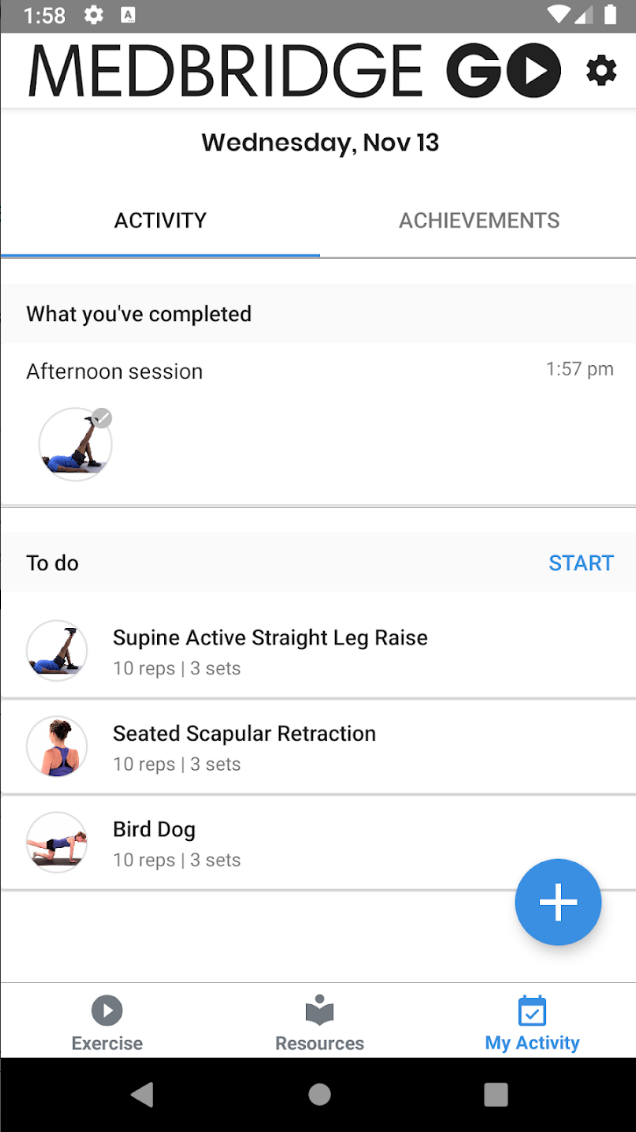
\includegraphics[width=0.35\linewidth]{slike/medbridge-go.png}
                            \caption{Sučelje aplikacije Medbridge GO koja je dostupna na pametnim telefonima}
                        \end{figure}
                        \item \textbf{BokDoc i BokDoc Partner:} Aplikacijski paket namijenjen rezervaciji termina kod doktora te promociji različitih privatnih klinika. Izgleda kao hibrid društvene mreže i oglasnika s mogućnošću narudžbe. Isto nije slična našem proizvodu. 
                        Ponovno postoje različiti profili za liječnika i pacijenta, ovoga puta to su potpuno različite aplikacije.  
                        \FloatBarrier
                        \begin{figure}
                            \centering
                            
\includegraphics[width=0.35\linewidth]{slike/BokDoc.png}
                            \caption{Sučelje aplikacije BokDoc koja je dostupna na pametnim telefonima}
                        \end{figure}
                        \FloatBarrier
                        \item \textbf{Practo:} Indijska telemedicinska aplikacija koja nudi različite zdravstvene usluge. Uključuje video konzultacije, online zakazivanje, pronalazak bolnica i tretmana te čitanje zdravstvenih savjeta. Velika mreža liječnika i pružatelja zdravstvenih usluga dostupna je korisnicima. 
                        Razlikuje se od našeg proizvoda jer se fokusira na širok spektar zdravstvenih usluga, dok je naša aplikacija specifična za upravljanje procesima rehabilitacije.
                        \FloatBarrier
                        \begin{figure}[!h]
                            \centering
                            
\includegraphics[width=0.5\linewidth]{slike/Practo.png}
                            \caption{Sučelje aplikacije Practo, dostupno na pametnim telefonima}
                        \end{figure}
                        \FloatBarrier
                        \item \textbf{SimplyBook.me i SimplyBook.me Admin:} SimplyBook.me je aplikacija za upravljanje terminima, posebno prilagođena korisnicima koji žele lagan pristup svojim postojećim rezervacijama. Omogućuje jednostavno dodavanje klijenata i uređivanje starih rezervacija. Korisnici primaju obavijesti o novim rezervacijama i podsjetnike za nadolazeće termine. Aplikacija je idealna za korisnike koji su često u pokretu, nemaju pristup uređajima s velikim ekranima tijekom radnog vremena ili žele provjeriti nadolazeće termine dok su kod kuće. Razlikuje se od našeg proizvoda jer je usmjerena na općenito upravljanje terminima, dok se naša aplikacija fokusira na specifične potrebe procesa rehabilitacije u zdravstvenim ustanovama.
                        \FloatBarrier
                        \begin{figure}[!h]
                            \centering
                            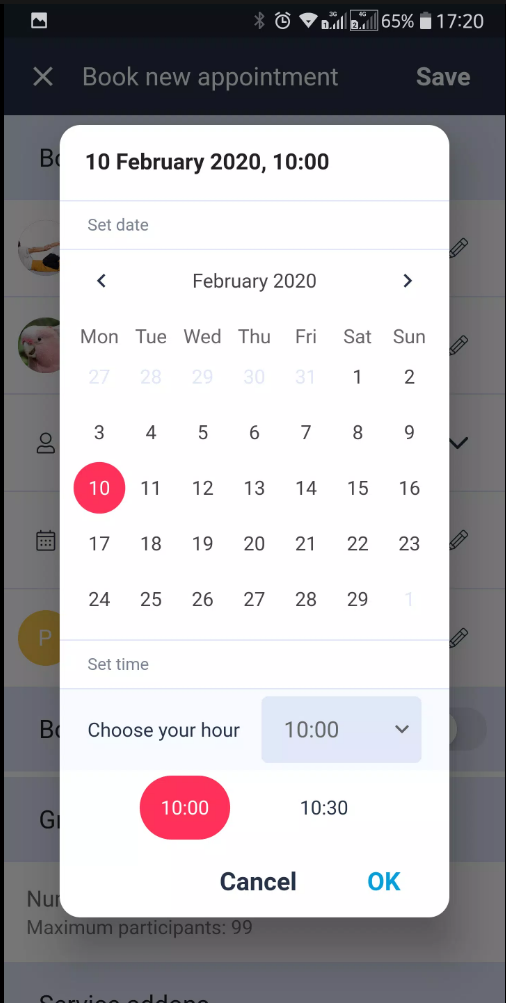
\includegraphics[width=0.45\linewidth]{slike/simplybook-client.png}
                            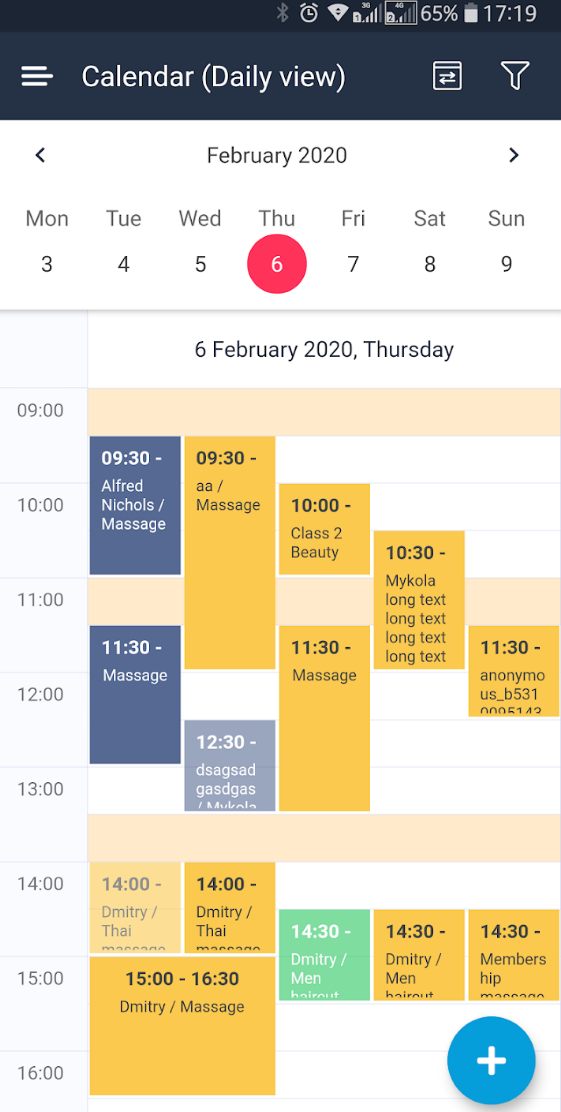
\includegraphics[width=0.45\linewidth]{slike/simplybook-admin.png}
                            \caption{Sučelje aplikacije SimplyBook.me: lijevo - korisnički pogled, desno - admin pogled}
                        \end{figure}
                        \FloatBarrier

                    \end{itemize}

                \end{itemize}


        
  
		\section*{Zaključak}

        Projekt koji smo razvili predstavlja potencijalni korak prema poboljšanju sustava rehabilitacije unutar zdravstvenog sektora. Naša aplikacija nudi inovativno rješenje koje se bavi ključnim izazovima učinkovitog upravljanja terminima i procesima, a posebno je prilagođena specifičnostima hrvatskog zdravstvenog sustava.
        
        \begin{itemize}
            \item \textbf{Inovativni pristup:} Transformacijom manualnih procesa u digitaliziranu, automatiziranu platformu aplikacija donosi povećanu efikasnost, transparentnost i bolje iskorištavanje resursa. To ne samo da unapređuje iskustvo pacijenata, već i olakšava posao djelatnicima i administratorima.
            
            \item \textbf{Fokus na korisnicima:} Razvojem aplikacije s jasnim fokusom na potrebe i udobnost korisnika posebno smo se posvetili stvaranju intuitivnog sučelja koje je pristupačno i jednostavno za korištenje svim dionicima procesa rehabilitacije.
        
            \item \textbf{Prilagodljivost i skalabilnost:} Projekt je dizajniran s obzirom na buduću ekspanziju i prilagodbu. Hibridni pristup razvoja aplikacije omogućava nam da odgovorimo na različite potrebe i zahtjeve različitih zdravstvenih ustanova nudeći im prilagođeno rješenje dok istovremeno zadržavamo unificiranu, centraliziranu strukturu.
        
            \item \textbf{Doprinos zdravstvu:} Ova aplikacija ima potencijal da značajno doprinese hrvatskom zdravstvenom sustavu koji bi osuvremenila glede procesa rehabilitacije što će imati dugoročne pozitivne učinke na kvalitetu zdravstvene skrbi.
        \end{itemize}
        
        Zaključno, ovaj projekt predstavlja važan korak naprijed u digitalizaciji zdravstvenih procesa s potencijalom da unese značajne promjene u načinu na koji se upravlja rehabilitacijom i srodnim zdravstvenim uslugama. Kroz kontinuirani razvoj i prilagodbu, ovaj sustav može služiti kao model za buduće inovacije unutar zdravstvenog sektora.
        
		
		\eject
		
	

	\chapter{Specifikacija programske potpore}

\section{Funkcionalni zahtjevi}

% Define a counter for use cases
\newcounter{UCCounter}

% Define a command for beginning a new use case
\newcommand{\usecase}[1]{
  \refstepcounter{UCCounter} % Increment the counter
  \noindent\underbar{\textbf{UC\theUCCounter{} - #1}} % Print the use case title with the number
  \begin{packed_item}
}

% Define a command for ending a use case
\newcommand{\closeusecase}{
  \end{packed_item}
  \vspace{1em}
}

\textbf{\textit{dio 1. revizije}}

\textit{ Glavni dionici su bolesnici, djelatnici zdravstvene ustanove te administratori sustava. Bolesnici su krajnji korisnici koji se prijavljuju na rehabilitaciju. Djelatnici zdravstvene ustanove provode rehabilitaciju i upravljaju terminima. Administratori sustava nadziru cjelokupno funkcioniranje sustava i upravljaju korisnicima.}


\noindent \textbf{Dionici:}

\begin{packed_enum}

	\item Administrator
	\item Djelatnik
	\item Bolesnik

\end{packed_enum}

\noindent \textbf{Aktori i njihovi funkcionalni zahtjevi:}


\begin{packed_enum}
	\item  \underbar{Administrator može:}

	\begin{packed_enum}

        \item Prijaviti se u sustav 
	\item Prihvatiti ili odbiti registraciju bolesnika
        \item Pregledati i potvrditi prijave bolesnika za rehabilitaciju
        \item Pregledati sve termine sesija
        \item Dodavati račune djelatnika
        \item Brisati račune bolesnika i djelatnika
        \item Pregledavati, uređivati i brisati podatke računa bolesnika i djelatnika
        \item Otkazati zakazani termin 
        \item Pomicati zakazane termine 

	\end{packed_enum}

	\item  \underbar{Djelatnik može:}

	\begin{packed_enum}

        	\item Prijaviti se u sustav 
		\item Bilježiti napredak svojih bolesnika
		\item Pregledati raspored svojih sesija
		\item Pregledati podatke o bolesnicima
		\item Otkazati sesiju pod određenim uvjetima

	\end{packed_enum}

	\item \underbar{Bolesnik može:}

	\begin{packed_enum}

		\item Registrirati se u sustav
        	\item Prijaviti se u sustav 
		\item Prijaviti se na rehabilitaciju
		\item Odabrati terapiju i termine dolaska na rehabilitaciju
		\item Pomaknuti zakazani termin pod određenim uvjetima
		\item Pregledati vlastiti kalendar s terminima terapije
		\item Pregledati povijest svojih terapija 
  

	\end{packed_enum}

	\item \underbar{Baza podataka:}

	\begin{packed_enum}

		\item Pohranjuje sve podatke o bolesnicima i njihovim rehabilitacijama
		\item Pohranjuje sve potrebne podatke o djelatnicima i njihovim terminima
       		\item Pohranjuje podatke o resursima ustanove 

	\end{packed_enum}
\end{packed_enum}

\eject



\subsection{Obrasci uporabe}

\textbf{\textit{dio 1. revizije}}

\subsubsection{Opis obrazaca uporabe}
\textit{Funkcionalne zahtjeve razraditi u obliku obrazaca uporabe. Svaki obrazac je potrebno razraditi prema donjem predlošku. Ukoliko u nekom koraku može doći do odstupanja, potrebno je to odstupanje opisati i po mogućnosti ponuditi rješenje kojim bi se tijek obrasca vratio na osnovni tijek.}
\vspace{2em} % Dodajte jedan prazan red

\usecase{Zahtjev za registraciju bolesnika u sustav}
	\item \textbf{Glavni sudionik:} Bolesnik
	\item \textbf{Cilj:} Poslati ispravan zahtjev za registraciju u sustav kako bi pristupio procesu rehabilitacije.
	\item \textbf{Sudionici:} Baza podataka
	\item \textbf{Preduvjet:} Bolesnik nema prethodno registriran korisnički račun
	\item \textbf{Opis osnovnog tijeka:}
	\begin{packed_enum}
		\item Bolesnik unosi osobne podatke, adresu elektroničke pošte i lozinku.
	\end{packed_enum}
\closeusecase


\usecase{Potvrda registracije bolesnika u sustav}
	\item \textbf{Glavni sudionik:} Administrator
	\item \textbf{Cilj:} Provjeriti i potvrditi registraciju bolesnika.
	\item \textbf{Sudionici:} Baza podataka, Bolesnik
	\item \textbf{Preduvjet:} Bolesnik je prethodno poslao zahtjev za registraciju, administrator je prijavljen u sustav.
	\item \textbf{Opis osnovnog tijeka:}
	\begin{packed_enum}
		\item Administrator provjerava ispravnost podataka.
		\item Sustav pohranjuje podatke i stvara korisnički račun.
  		\item Bolesnik prima elektroničku poštu s potvrdom registracije.
	\end{packed_enum}
	\item \textbf{Opis mogućih odstupanja:}
	U slučaju neispravne registracije u smislu duplikata OIB-a ili MBO-a frontend ne dopušta slanje registracije. 
    	Ukoliko nepravilnosti uoči administrator, Bolesnik prima elektroničku poštu na upisanu adresu u kojoj mu se govori da registracija nije uspjela.
\closeusecase


\usecase{Prijava bolesnika/djelatnika/administratora u sustav}
	\item \textbf{Glavni sudionik:} Bolesnik/Djelatnik/Administrator
	\item \textbf{Cilj:} Korisnik se želi prijaviti u sustav 
	\item \textbf{Sudionici:} Baza podataka
	\item \textbf{Preduvjet:} Korisnikov račun je u bazi podataka
	\item \textbf{Opis osnovnog tijeka:}
	\begin{packed_enum}
		\item Korisnik unosi adresu elektroničke pošte i lozinku.
		\item Provjerava se postojanost dane kombinacije u bazi
		\item Ovisno o tipu profila povezanog s unesenim podacima, korisniku se otvara jedno od 3 moguća sučelja (bolesnik, djelatnik, administrator)
	\end{packed_enum}
	\item \textbf{Opis mogućih odstupanja:}
	Sustav reagira na neispravne podatke te obavještava korisnika o netočnosti podataka. \\
\closeusecase


\usecase{Zaboravljena lozinka za prijavu}
	\item \textbf{Glavni sudionik:} Bolesnik/Djelatnik/Administrator
 	\item \textbf{Cilj:} Prijaviti se unatoč zaboravljenoj lozinci
  	\item \textbf{Sudionici:} Baza podataka
   	\item \textbf{Preduvjet:} Korisnikova e-mail adresa je u bazi podataka
    	\item \textbf{Opis osnovnog tijeka:}
     	\begin{packed_enum}
      		\item Korisnik je zaboravio lozinku te se ne može prijaviti u sustav
		\item Korisnik pritišće gumb za dobivanje nove lozinke
  		\item Korisnik na e-mail adresu dobiva upute za postavljanje nove lozinke
    	\end{packed_enum}
\closeusecase


\usecase{Prijava bolesnika na rehabilitaciju}
	\item \textbf{Glavni sudionik:} Bolesnik
	\item \textbf{Cilj:} Prijaviti se za proces rehabilitacije.
	\item \textbf{Sudionici:} Baza podataka
	\item \textbf{Preduvjet:} Bolesnik je registriran i prijavljen u sustav.
	\item \textbf{Opis osnovnog tijeka:}
	\begin{packed_enum}
		\item Bolesnik odabire opciju za prijavu na rehabilitaciju.
		\item Bolesnik unosi informacije o svom oboljenju, potrebnom postupku liječenja i liječniku koji ga je uputio na rehabilitaciju.
        	\item S obzirom na unesenu vrstu rehabilitacije, sustav provjerava koji su sve termini slobodni (slobodan termin: slobodan resurs i slobodan specijalizirani djelatnik) 
		\item Bolesnik odabire datum i vrijeme svojih termina na temelju dostupnih termina 
        	\item Bolesnik čeka odobrenje administratora (UCXY) 
        	\item Korisnik prima skočni prozor s obavijesti o administratorovoj odluci te sukladno istoj ili može ponoviti prijavu na rehabilitaciju ili je preusmjeren na kontrolnu ploču (dashboard) za novonastalu rehabilitaciju
	\end{packed_enum}
	\item \textbf{Opis mogućih odstupanja:}
	Dok sve nužne informacije nisu upisane blokirano je slanje forme na provjeru kod administratora. 
\closeusecase


\usecase{Promjena zakazanog termina (bolesnik)}
	\item \textbf{Glavni sudionik:} Bolesnik
	\item \textbf{Cilj:} Promijeniti zakazani termin za rehabilitaciju.
	\item \textbf{Sudionici:} Baza podataka
	\item \textbf{Preduvjet:} Bolesnik je registriran, prijavljen i ima zakazane termine.
	\item \textbf{Opis osnovnog tijeka:}
	\begin{packed_enum}
        	\item Bolesnik ulazi na kontrolnu ploču.
	 	\item Bolesnik pregledava svoj raspored i odabire termin koji bi htio promijeniti.
		\item Bolesnik u informacijama o terminu odabire opciju za promjenu termina.
		\item Bolesnik pregledava raspored slobodnih termina i odabire zamjenski termin.
		\item Sustav potvrđuje regularnost promjene i ona se evidentira na kontrolnoj ploči djelatnika i bolesnika. 
	\end{packed_enum}
    	\item \textbf{Opis mogućih odstupanja:}
		Ako promjena nije napravljena minimalno 48 sati prije termina, otkazivanja su onemogućena u sustavu i bolesnik se upućuje da u slučaju hitnosti kontaktira administratora direktno. 
\closeusecase


\usecase{Pregled relevantnih informacija za budući termin}
	\item \textbf{Glavni sudionik:} Bolesnik
 	\item \textbf{Cilj:} Dobiti više informacija o određenom terminu
  	\item \textbf{Sudionici:} Baza podataka
   	\item \textbf{Preduvjet:} Korisnik je prijavljen u sustav, prijavljen na terapiju i ima barem jedan preostali termin
    	\item \textbf{Opis osnovnog tijeka:}
     	\begin{packed_enum}
      		\item Korisnik na svojem rasporedu odabire jedan termin
		\item Korisnik pritišće gumb "Prikaži više" za taj termin
  		\item Korisniku se pojavljuje novi prozor s informacijama o terminu kao što su broj sesije, opis sesije, ime djelatnika te mapa ustanove s naznačenim mjestom odvijanja te sesije
    	\end{packed_enum}
\closeusecase


\usecase{Otkazivanje zakazanog termina (djelatnik)}
	\item \textbf{Glavni sudionik:} Djelatnik
	\item \textbf{Cilj:} Otkazati zakazani termin za rehabilitaciju.
	\item \textbf{Sudionici:} Baza podataka
	\item \textbf{Preduvjet:} Djelatnik je prijavljen u sustav. Bolesnik ima zakazane termine.
	\item \textbf{Opis osnovnog tijeka:}
	\begin{packed_enum}
        	\item Djelatnik ulazi na kontrolnu ploču i odabire termin koji želi promijeniti.
		\item Djelatnik odabire opciju za otkazivanje termina 
        	\item Izvršava se promjena u bazi te se obavještava bolesnik koji odabire novi termin 
	\end{packed_enum}
    \item \textbf{Opis mogućih odstupanja:}
	Djelatnik ne može otkazivati termine koji nisu njegovi. 
\closeusecase


\usecase{Otkazivanje zakazanog termina (administrator)}
	\item \textbf{Glavni sudionik:} Administrator
	\item \textbf{Cilj:} Otkazati zakazani termin za rehabilitaciju.
	\item \textbf{Sudionici:} Baza podataka
	\item \textbf{Preduvjet:} Administrator je prijavljen u sustav. Bolesnik ima zakazane termine.
	\item \textbf{Opis osnovnog tijeka:}
	\begin{packed_enum}
        	\item Administrator odlazi na kalendar i pretražuje termin po djelatniku i/ili po bolesniku.
		\item Administrator odabire opciju za otkazivanje termina 
        	\item Izvršava se promjena u bazi te se obavještava djelatnika i bolesnika koji odabire novi termin 
	\end{packed_enum}
\closeusecase


\usecase{Pregled kalendara vlastitih terapija}
	\item \textbf{Glavni sudionik:} Bolesnik/Djelatnik
	\item \textbf{Cilj:} Pregledati kalendar s terminima terapije.
	\item \textbf{Sudionici:} Baza podataka
	\item \textbf{Preduvjet:} Bolesnik/Djelatnik je registriran i prijavljen u sustav.
	\item \textbf{Opis osnovnog tijeka:}
	\begin{packed_enum}
		\item Bolesnik/Djelatnik odabire opciju za pregled vlastitog kalendara.
		\item Sustav prikazuje raspored svih zakazanih termina terapije.
        	\item Bolesnik može pregledati sesije i vidjeti napomene, djelatnik ih može upisivati
	\end{packed_enum}
\closeusecase


\usecase{Pregled podataka o bolesnicima}
	\item \textbf{Glavni sudionik:} Djelatnik
	\item \textbf{Cilj:} Pregledati podatke o bolesnicima.
	\item \textbf{Sudionici:} Baza podataka
	\item \textbf{Preduvjet:} Djelatnik je prijavljen u sustav.
	\item \textbf{Opis osnovnog tijeka:}
	\begin{packed_enum}
		\item Djelatnik pretražuje ime bolesnika ili pregledava listu svih bolesnika.
		\item Sustav prikazuje popis bolesnika i osnovne informacije o njima.
		\item Djelatnik može pregledati detaljnije podatke o svakom bolesniku.
	\end{packed_enum}
\closeusecase


\usecase{Pregled rasporeda svih bolesnika, djelatnika i sesija}
	\item \textbf{Glavni sudionik:} Administrator
	\item \textbf{Cilj:} Pregledati raspored bolesnika i sesija rehabilitacije.
	\item \textbf{Sudionici:} Baza podataka
	\item \textbf{Preduvjet:} Administrator je prijavljen u sustav.
	\item \textbf{Opis osnovnog tijeka:}
	\begin{packed_enum}
		\item Administrator odabire opciju za pregled rasporeda.
		\item Sustav prikazuje raspored svih bolesnika, djelatnika i sesija.
		\item Administrator može filtrirati raspored po različitim kriterijima.
	\end{packed_enum}
\closeusecase


\usecase{Bilježenje napretka bolesnika}
	\item \textbf{Glavni sudionik:} Djelatnik
	\item \textbf{Cilj:} Bilježiti i evidentirati napredak bolesnika tijekom procesa rehabilitacije.
	\item \textbf{Sudionici:} Baza podataka
	\item \textbf{Preduvjet:} Bolesnik je registriran, prijavljen i odradio sesiju rehabilitacije s određenim djelatnikom.
	\item \textbf{Opis osnovnog tijeka:}
	\begin{packed_enum}
		\item Djelatnik odabire bolesnika za bilježenje napretka.
		\item Djelatnik unosi podatke o sesiji rehabilitacije.
		\item Djelatnik potvrđuje unos i sprema podatke.
	\end{packed_enum}
\closeusecase


\usecase{Pregled podataka o terapijama}
	\item \textbf{Glavni sudionik:} Bolesnik
	\item \textbf{Cilj:} Pregledati podatke o terapijama.
	\item \textbf{Sudionici:} Baza podataka
	\item \textbf{Preduvjet:} Bolesnik je registriran i prijavljen u sustav.
	\item \textbf{Opis osnovnog tijeka:}
	\begin{packed_enum}
		\item Bolesnik odabire opciju za pregled podataka.
		\item Sustav prikazuje relevantne informacije o terapijama.
	\end{packed_enum}
\closeusecase


\usecase{Pregled statistike o djelatnicima i resursima}
	\item \textbf{Glavni sudionik:} Administrator 
	\item \textbf{Cilj:} Praćenje dostupnosti osoblja, opreme i kapaciteta za rehabilitaciju.
	\item \textbf{Sudionici:} Baza podataka
	\item \textbf{Preduvjet:} Administrator je prijavljen u sustav.
	\item \textbf{Opis osnovnog tijeka:}
	\begin{packed_enum}
		\item Administrator iz kontrolne ploče odabire Pregled statistike o djelatnicima i resursima
		\item Sustav prikazuje zadani pogled (eng. view). 
	\end{packed_enum}
\closeusecase


\usecase{Dodavanje djelatnika u bazu}
	\item \textbf{Glavni sudionik:} Administrator
	\item \textbf{Cilj:} Stvoriti korisnički račun za novog djelatnika u sustavu medicinske rehabilitacije.
	\item \textbf{Sudionici:} Baza podataka
	\item \textbf{Preduvjet:} Administrator je prijavljen u sustav.
	\item \textbf{Opis osnovnog tijeka:}
	\begin{packed_enum}
		\item Administrator iz kontrolne ploče odabire opciju za stvaranje novog djelatnika.
		\item Sustav prikazuje obrazac za unos osobnih podataka novog djelatnika.
		\item Administrator unosi sve potrebne podatke o novom djelatniku.
		\item Ako su svi podaci ispravni, sustav stvara novi korisnički račun za djelatnika.
	\end{packed_enum}
	\item \textbf{Opis mogućih odstupanja:}
	Sustav reagira na neispravne podatke, već postojeće zaposlenike te obavještava administratora o neuspjelom upisu.
\closeusecase


\usecase{Promjena podataka o djelatnicima i bolesnicima}
	\item \textbf{Glavni sudionik:} Administrator
	\item \textbf{Cilj:} Izmijeniti informacije o djelatnicima i bolesnicima u bazi.
	\item \textbf{Sudionici:} Baza podataka
	\item \textbf{Preduvjet:} Administrator je prijavljen u sustav.
	\item \textbf{Opis osnovnog tijeka:}
	\begin{packed_enum}
		\item Administrator iz kontrolne ploče odabire pregled svih djelatnika ili bolesnika.
		\item Administrator odabire djelatnika/bolesnika i uređuje informacije o istom.
        	\item Prije potvrde o promjeni administrator ponovno unosi svoju šifru
	\end{packed_enum}
\closeusecase


\usecase{Deaktivacija korisničkog računa djelatnika/bolesnika}
	\item \textbf{Glavni sudionik:} Administrator
	\item \textbf{Cilj:} Deaktivirati korisnički račun djelatnika/bolesnika.
	\item \textbf{Sudionici:} Baza podataka
	\item \textbf{Preduvjet:} Administrator je prijavljen u sustav.
	\item \textbf{Opis osnovnog tijeka:}
	\begin{packed_enum}
		\item Administrator iz kontrolne ploče odabire pregled svih djelatnika ili bolesnika.
		\item Administrator odabire djelatnika/bolesnika čiji korisnički račun želi deaktivirati.
        	\item Prije potvrde o promjeni administrator ponovno unosi svoju šifru
	\end{packed_enum}
\closeusecase


\usecase{Deaktivacija vlastitog korisničkog računa}
	\item \textbf{Glavni sudionik:} Bolesnik
	\item \textbf{Cilj:} Deaktivirati vlastiti korisnički račun.
	\item \textbf{Sudionici:} Baza podataka
	\item \textbf{Preduvjet:} Bolesnik je prijavljen u sustav.
	\item \textbf{Opis osnovnog tijeka:}
	\begin{packed_enum}
		\item Bolesnik odabire opciju za deaktivaciju računa.
		\item Sustav traži bolesnikovu lozinku za potvrdu zahtjeva.
		\item Sustav je deaktivirao bolesnikov korisnički račun.
	\end{packed_enum}
	\item \textbf{Opis mogućih odstupanja:}
	Sustav reagira na neispravnu lozinku te obavještava bolesnika o neuspjelom pokušaju.
\closeusecase


\subsubsection{Dijagrami obrazaca uporabe}

\textit{Prikazati odnos aktora i obrazaca uporabe odgovarajućim UML dijagramom. Nije nužno nacrtati sve na jednom dijagramu. Modelirati po razinama apstrakcije i skupovima srodnih funkcionalnosti.}
\eject

\subsection{Sekvencijski dijagrami}

\textbf{\textit{dio 1. revizije}}\\

\textit{Nacrtati sekvencijske dijagrame koji modeliraju najvažnije dijelove sustava (max. 4 dijagrama). Ukoliko postoji nedoumica oko odabira, razjasniti s asistentom. Uz svaki dijagram napisati detaljni opis dijagrama.}
\eject

\section{Ostali zahtjevi}

\textbf{\textit{dio 1. revizije}}\\

\textit{Nefunkcionalni zahtjevi i zahtjevi domene primjene dopunjuju funkcionalne zahtjeve. Oni opisuju \textbf{kako se sustav treba ponašati} i koja \textbf{ograničenja} treba poštivati (performanse, korisničko iskustvo, pouzdanost, standardi kvalitete, sigurnost...). Primjeri takvih zahtjeva u Vašem projektu mogu biti: podržani jezici korisničkog sučelja, vrijeme odziva, najveći mogući podržani broj korisnika, podržane web/mobilne platforme, razina zaštite (protokoli komunikacije, kriptiranje...)... Svaki takav zahtjev potrebno je navesti u jednoj ili dvije rečenice.}
			 
			 
			 
	

	\chapter{Arhitektura i dizajn sustava}

\textbf{\textit{dio 1. revizije}}\\

\section*{Uvod u Arhitekturu Sustava}
Naš sustav je dizajniran da bude efikasan, skalabilan i pouzdan. U nastavku detaljno opisujemo arhitekturu našeg sustava.

\subsection*{Izbor Arhitekture}
\begin{itemize}
    \item Naša odluka da koristimo trodijelnu arhitekturu temelji se na principima oblikovanja predstavljenim na predavanjima, gdje se ističe važnost modularnosti i odvajanja odgovornosti. Ovaj temeljni pristup oblikovanju sustava reflektira našu predanost stvaranju arhitekture koja je ne samo funkcionalna, već i prilagodljiva, jednostavna za održavanje te otporna na buduće izazove. 

    \item Princip modularnosti naglašava važnost razdvajanja sustava na manje, samostalne dijelove, ili module. Ovakav pristup omogućava da svaki modul ima jasno definiranu funkcionalnost, što pojednostavljuje razvoj, testiranje i održavanje. Svaki modul može biti razvijen neovisno, što pridonosi većoj fleksibilnosti i olakšava integraciju novih značajki ili promjena u sustavu. 

    \item Odvajanje odgovornosti, s druge strane, znači da svaki dio sustava ima precizno definiranu ulogu ili odgovornost. Na primjer, frontend se odvaja od backenda, čime se postiže jasna granica između korisničkog sučelja i poslovne logike. Ovo olakšava praćenje i održavanje svake komponente zasebno, smanjuje rizik od pogrešaka i omogućava paralelno razvijanje dijelova sustava. 

\item Trodijelna arhitektura, koja obuhvaća backend, frontend i bazu podataka, idealno se uklapa u ove principe. Backend je odgovoran za poslovnu logiku, frontend za korisničko sučelje, dok je baza podataka centralno mjesto za pohranu podataka. Ovaj pristup omogućava svakom dijelu sustava da obavlja svoju specifičnu funkciju, čime se postiže bolja organizacija, održavanje i skalabilnost. 

\subsection*{Organizacija Sustava}
\item Naš sustav je pažljivo organiziran na visokoj razini apstrakcije, koristeći klijent-poslužitelj model, što predstavlja ključni element naše arhitekture. Ova organizacija ima za cilj efikasno upravljanje različitim dijelovima sustava, pružajući jasno odvojeni pristup korisničkom sučelju i poslovnoj logici. 

\item \textbf{Klijent-poslužitelj} model je arhitektonski oblik koji omogućuje razdvajanje funkcionalnosti između dviju osnovnih komponenti: klijenta i poslužitelja. Klijent predstavlja korisničko sučelje, dok poslužitelj sadrži poslovnu logiku i podatke. Ovaj model omogućuje svakoj komponenti da obavlja svoje specifične zadatke, što rezultira modularnošću i skalabilnošću sustava. 

\textbf{Prednosti klijent-poslužitelj modela:}

\begin{enumerate}
    \item Razdvajanje odgovornosti: Klijent i poslužitelj imaju jasno definirane uloge, čime se postiže precizno odvajanje korisničkog sučelja od poslovne logike. To olakšava održavanje, poboljšava sigurnost i doprinosi boljoj organizaciji koda.
    \item Fleksibilnost i skalabilnost: Modularnost klijent-poslužitelj arhitekture omogućava prilagodbu svake komponente neovisno. Na primjer, možemo nadograditi ili zamijeniti korisničko sučelje bez narušavanja poslovne logike i obrnuto. Ovo čini sustav fleksibilnim i lako skalabilnim.
    \item Efikasna komunikacija: Klijent i poslužitelj komuniciraju putem standardiziranih protokola, često kroz HTTP. Ova jasna komunikacija omogućava brzu i pouzdanu razmjenu podataka između dijelova sustava.
\end{enumerate}
 
Odvajanje korisničkog sučelja od poslovne logike donosi dodatne prednosti. Korisničko sučelje, koje može biti web aplikacija ili mobilna aplikacija, fokusira se na prezentaciju podataka i interakciju s korisnicima. S druge strane, poslovna logika centralizirana je na poslužitelju, gdje se vrše obrade podataka, donose poslovne odluke i upravlja cjelokupnim tokom aplikacije. 

\subsection*{Detalji Podsustava}
\subsubsection*{Backend (Spring Boot)}
\item Backend predstavlja ključnu osnovu našeg sustava, pružajući infrastrukturu za obradu poslovnih zahtjeva. Organiziran je kao skup podsustava, uključujući servise i kontrolere, čija je svrha efikasno rukovanje različitim aspektima poslovnih funkcionalnosti.

\textbf{Servisi}: Funkcionalne jedinice sustava odgovorne za izvođenje specifičnih poslovnih operacija. Svaki servis fokusira se na određenu funkcionalnost, pridonoseći modularnosti i omogućavajući bolje upravljanje kompleksnošću sustava. Na primjer, možemo imati servis za korisničke operacije, proizvode ili neki drugi poslovni entitet.\newline
\textbf{Kontroleri}: Odgovorni za obradu i usmjeravanje HTTP zahtjeva koji dolaze od klijenata. Kontroleri predstavljaju sučelje između korisničkog sučelja (frontend) i poslovnih operacija koje izvode servisi. Ovo odvajanje odgovornosti omogućava bolju organizaciju koda i olakšava testiranje.



\textbf{Komunikacija s bazom podataka (PostgreSQL):}
\item Backend komunicira s bazom podataka putem PostgreSQL sustava, koji omogućava efikasnu organizaciju i manipulaciju podacima zbog svoje pouzdane i robusne arhitekture. Relacijski model podataka pruža strukturu temeljenu na tablicama, što olakšava povezivanje podataka između različitih dijelova sustava.
    \item Ovaj pristup omogućava lako preslikavanje podataka iz aplikacije u bazu i obrnuto, pridonoseći dosljednosti podataka i olakšavajući njihovo upravljanje. Kroz PostgreSQL, ostvarujemo centralno spremište podataka koje je ključno za sve relevantne informacije u sustavu.
\end{itemize}
Backend, kao središnja komponenta sustava, osigurava da poslovna logika bude učinkovito izvršavana, a podaci pravilno organizirani i održavani. Ovaj dio arhitekture pridonosi integraciji svih poslovnih funkcionalnosti, čime se postiže koherentan i efikasan rad sustava.\newline

 
 

\textbf{Frontend (Node.js, JavaScript, React)}
Frontend, kao ključna korisnička strana našeg sustava, organiziran je prema modernim principima razvoja web aplikacija. Glavni tehnološki alati koje koristimo su Node.js, JavaScript i React, pružajući nam moćne alate za stvaranje fleksibilnog i intuitivnog korisničkog sučelja.

Organizacija u komponente i kontejnere:

\begin{itemize}
    \item Komponente su modularni dijelovi koji obavljaju specifične zadatke, kao što su prikazivanje određenih podataka ili omogućavanje korisničkih interakcija.
    \item Kontejneri služe kao viši slojevi koji upravljaju komponentama, pružajući organiziran pristup i poboljšavajući skalabilnost.

\end{itemize}
REST API za komunikaciju s backendom:

\begin{itemize}
    \item Frontend komunicira s backendom putem REST API-ja (Representational State Transfer), standardnog protokola za komunikaciju između klijenta i poslužitelja koji omogućava brzu, standardiziranu i pouzdanu razmjenu podataka između frontend i backend dijelova sustava.
\end{itemize}
React kao glavni framework:

\begin{itemize}
    \item Koristimo React, popularni JavaScript framework za izgradnju korisničkih sučelja. React omogućava brzo renderiranje stranica, poboljšava učinkovitost i olakšava manipulaciju komponentama.
    \item Kroz React, frontend postaje reaktivno sučelje koje brzo reagira na promjene stanja podataka, pružajući korisnicima ugodno iskustvo korištenja aplikacije.
\end{itemize}

 

\subsubsection*{Baza podataka (PostgreSQL)}
\begin{itemize}
    \item Baza podataka predstavlja ključnu komponentu našeg sustava, pružajući centralno spremište za sve relevantne podatke. 
    \item U našem slučaju, koristimo PostgreSQL, robustan i napredan relacijski sustav upravljanja bazama podataka, kako bismo osigurali pouzdanu pohranu i učinkovit pristup podacima. 
    \item Struktura baze je dizajnirana da podržava složene upite i relacije između različitih podataka.
\end{itemize}

\subsection*{Mrežni Protokoli i Komunikacija}
\begin{itemize}
    \item Komunikacija između klijenta i poslužitelja odvija se preko HTTP protokola, osiguravajući sigurnost i standardiziran protok informacija.
    \item Kroz HTTP, klijent šalje zahtjeve poslužitelju, a poslužitelj šalje odgovore. 
\end{itemize}

\subsection*{Globalni Upravljački Tok}
\begin{itemize}
    \item Globalni upravljački tok u našem sustavu određen je kroz primjenu MVC (Model-View-Controller) arhitekture, pružajući strukturu i organizaciju za učinkovitu interakciju između različitih dijelova aplikacije. 
\end{itemize}

\textbf{MVC Arhitektura:}

\begin{itemize}
    \item \textbf{Model}: Model predstavlja središnju komponentu sustava koja upravlja podacima. Ovdje se nalaze podaci i poslovna logika aplikacije. Model je odvojen od korisničkog sučelja i interakcije te služi kao zasebna jedinica koja obrađuje podatke neovisno o korisničkom sučelju.
    \item \textbf{View}: View je odgovoran za prikazivanje podataka korisnicima. Ova komponenta generira korisničko sučelje na temelju podataka iz Modela. View je pasivan i ne obavlja izravne operacije na podacima, već ih prikazuje korisnicima na razumljiv način.
    \item \textbf{Controller}: Controller predstavlja upravljački sloj koji obrađuje korisničke zahtjeve i interakcije. Kada korisnik obavi neku akciju, Controller reagira, a zatim komunicira s Modelom i Viewom prema potrebi. Ova komponenta osigurava odvajanje korisničkih akcija od same logike sustava.

\end{itemize}
\begin{figure}[h]
    \centering
    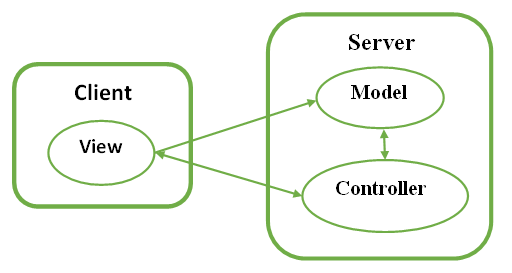
\includegraphics[width=0.5\linewidth]{slike/mvc2.png}
    \caption{MVC arhitektura}
    \label{fig:enter-label}
\end{figure}
 \textbf{
\newline Prednosti MVC Arhitekture:}
\begin{itemize}
    \item Odvajanje odgovornosti: MVC omogućava jasno odvajanje odgovornosti između različitih dijelova sustava. Model, View i Controller imaju specifične uloge, čime se olakšava razvoj, testiranje i održavanje koda.
    \item Lako proširivost i održavanje: Zbog modularnosti i odvajanja odgovornosti, dodavanje novih funkcionalnosti ili promjena postojećih dijelova sustava postaje jednostavno i manje riskantno.
    \item Jasna struktura: MVC pruža jasnu strukturu sustava, olakšavajući suradnju između različitih timova i programera. Ova organizacija doprinosi boljoj preglednosti i razumijevanju koda.
\end{itemize}

 
\subsection*{Sklopovsko-Programski Zahtjevi}
\begin{itemize}
    \item Integracijom sklopovsko-programskih zahtjeva, sustav omogućuje stabilnost te se uspješno priprema za izazove suvremenog informacijskog okruženja. 
\end{itemize}

\textbf{Prilagođenost modernim računalnim platformama:}
Sustav je optimiziran za rad na suvremenim računalnim platformama, uključujući njihove specifičnosti i prednosti. Koristeći najnovije tehnologije i prakse, osiguravamo kompatibilnost s različitim operativnim sustavima i konfiguracijama računala.\newline

\textbf{Visoka dostupnost:}
Dostupnost sustava ključna je za neprekidno pružanje usluga korisnicima. Implementiramo strategije visoke dostupnosti kako bismo osigurali minimalne prekide u radu sustava. Ovo uključuje redundanciju ključnih komponenti i mehanizme automatskog oporavka od mogućih kvarova.\newline


\textbf{Optimizacija performansi:}
Performanse su ključne za korisničko iskustvo i učinkovit rad sustava. Kroz optimizaciju koda, uporabu efikasnih algoritama i praćenje performansi u stvarnom vremenu, postižemo visoku razinu odziva i brze obrade podataka.\newline


\textbf{Prilagodljivost za skaliranje:}
Sustav je dizajniran kako bi se lako skalirao prema rastućim potrebama. Uz mogućnost horizontalnog i vertikalnog skaliranja, omogućujemo prilagodljivu infrastrukturu koja se može dinamički prilagoditi povećanju opterećenja.\newline

\textbf{Sigurnosni aspekti:}
Sklopovsko-programski zahtjevi također obuhvaćaju sigurnosne aspekte. Sustav implementira mjere zaštite podataka, enkripciju komunikacije i autentikaciju kako bi osigurao siguran rad i spriječio neovlašteni pristup.\newline


\textbf{Kontinuirano ažuriranje i praćenje trendova:}

S obzirom na brzu evoluciju tehnologije, sustav se kontinuirano prilagođava novim standardima i trendovima. Redovita ažuriranja omogućuju iskorištavanje najnovijih značajki, poboljšanje sigurnosti te održavanje konkurentske prednosti.\newline

Kroz integraciju navedenih sklopovsko-programskih zahtjeva, naš sustav ne samo da osigurava stabilnost i performanse, već je i spreman suočiti se s izazovima suvremenog informacijskog okruženja. Ovaj pristup jamči dugoročnu održivost, skalabilnost i optimalno iskorištavanje resursa računalnih platformi.

 


        \section{Baza podataka}
			
			\textbf{\textit{dio 1. revizije}}\\
			
Baza podataka predstavlja ključnu komponentu našeg sustava, pružajući centralno spremište za sve relevantne podatke. U našem slučaju, koristimo PostgreSQL, relacijski sustav upravljanja bazama podataka. PostgreSQL je snažan i visoko prilagodljiv sustav za upravljanje bazama podataka, što ga čini prikladnim izborom za učinkovito i sigurno upravljanje zdravstvenim podacima, osiguravajući da su informacije o pacijentima, terminima, zdravstvenom osoblju i opremi sigurno pohranjene i dostupne. 



\textbf{Pouzdana pohrana i pristup podacima:}

PostgreSQL pruža visoku razinu pouzdanosti i integriteta podataka. Njegova transakcijska podrška osigurava dosljednost podataka čak i u slučaju neplaniranih prekida rada sustava ili pogrešaka.
Centralizirano pohranjivanje podataka omogućava nam učinkovito upravljanje svim informacijama relevantnim za rad sustava.

\textbf{Struktura baze za složene upite i relacije:}
\begin{itemize}
\item Dizajn baze podataka ključan je za podršku složenim upitima i održavanje relacija između različitih podataka.
\item PostgreSQL, kao relacijski sustav, koristi tablice kako bi organizirao podatke. Svaka tablica sastoji se od redova i stupaca, omogućujući jasno definiranje veza između entiteta.
\item Veze između tablica omogućavaju složene upite koji spajaju informacije iz različitih dijelova sustava. 
PostgreSQL također podržava napredne mogućnosti poput indeksiranja, pomažući ubrzati upite i optimizirati performanse baze podataka.
\item  Struktura baze podataka je pažljivo oblikovana kako bi odražavala logičke relacije i potrebe sustava, čime se postiže efikasno upravljanje podacima.
\end{itemize}

		
			\subsection{Opis tablica}
			

				\textit{Svaku tablicu je potrebno opisati po zadanom predlošku. Lijevo se nalazi točno ime varijable u bazi podataka, u sredini se nalazi tip podataka, a desno se nalazi opis varijable. Svjetlozelenom bojom označite primarni ključ. Svjetlo plavom označite strani ključ}
				
\textbf{\_User } Ovaj entitet predstavlja korisnike sustava s različitim ulogama.  Sadrži atribute kao što su status korisnika (active), jedinstveni identifikator (id), e-mail adresa (email), ime (first\_name), prezime (last\_name), lozinka (password) i uloga korisnika (role). Provjerava se uloga korisnika kroz ograničenje \_user\_role\_check. Ovaj entitet omogućuje upravljanje korisnicima sustava i dodjeljivanje uloga kako bi se pristup određenim funkcionalnostima kontrolirao.  Primarni ključ (\_user\_pkey) je definiran na atributu id. 

\begin{longtblr}[
    label=none,
    entry=none
]{
    width = \textwidth,
    colspec={|X[6,l]|X[6, l]|X[20, l]|}, 
    rowhead = 1,
}
\hline \SetCell[c=3]{c}{\textbf{ \_user}} \\ \hline[3pt]
\SetCell{LightGreen}id & BIGINT & Jedinstveni identifikator korisnika \\ \hline
active & BOOLEAN & Označava je li korisnik aktivan \\ \hline 
email & VARCHAR & E-mail adresa korisnika \\ \hline 
first\_name & VARCHAR & Ime korisnika \\ \hline 
last\_name & VARCHAR & Prezime korisnika \\ \hline 
password & VARCHAR & Lozinka korisnika \\ \hline 
role & VARCHAR & Rola korisnika (mora biti jedna od predefiniranih uloga) \\ \hline 
\end{longtblr}

				
		
\textbf{Imenik} Entitet koji služi za pohranu informacija o liječnicima. Sadrži atribute kao što su jedinstveni identifikator liječnika (hlkid), ime (first\_name), prezime (last\_name), specijalizacija (specialization) i informacija o aktivnosti liječnika (active).  Primarni ključ (Imenik\_pkey) je definiran na atributu hlkid. 
\begin{longtblr}[
    label=none,
    entry=none
]{
    width = \textwidth,
    colspec={|X[6,l]|X[6, l]|X[20, l]|}, 
    rowhead = 1,
}
\hline \SetCell[c=3]{c}{\textbf{imenik}} \\ \hline[3pt]
\SetCell{LightGreen}hlkid & VARCHAR & Jedinstveni identifikator liječnika \\ \hline
first\_name & VARCHAR & Ime liječnika \\ \hline 
last\_name & VARCHAR & Prezime liječnika  \\ \hline 
specialization & VARCHAR & Specijalizacija liječnika  \\ \hline 
active & BOOLEAN & Označava je li liječnik u imeniku aktivna \\ \hline 
\end{longtblr}


\textbf{Appointment} Čuva informacije o terminima unutar sustava. Sadrži atribute kao što su datum i vrijeme termina (date\_time), identifikator zaposlenika (employee\_id), jedinstveni identifikator termina (id), identifikator pacijenta (patient\_id), identifikator sesije (session\_id), identifikator terapije (therapy\_id) i status termina (status). Ovaj entitet je povezan s drugim entitetima(employee, patient, session, therapy) putem različitih Many-to-One veza prema atributima \verb|employee_id|, \verb|patient_id|, \verb|session_id|, i \verb|therapy_id|. 

\begin{longtblr}[
    label=none,
    entry=none
]{
    width = \textwidth,
    colspec={|X[6,l]|X[6, l]|X[20, l]|}, 
    rowhead = 1,
}
\hline \SetCell[c=3]{c}{\textbf{appointment}} \\ \hline[3pt]
\SetCell{LightGreen}id & BIGINT & Jedinstveni identifikator termina \\ \hline 
date\_time & TIMESTAMP & Datum i vrijeme termina \\ \hline
\SetCell{LightBlue}employee\_id & BIGINT & Identifikator zaposlenika koji obavlja termin \\ \hline 
\SetCell{LightBlue}patient\_id & BIGINT & Identifikator pacijenta koji ima termin \\ \hline 
\SetCell{LightBlue}session\_id & BIGINT & Identifikator sesije kojoj pripada termin \\ \hline 
\SetCell{LightBlue}therapy\_id & BIGINT & Identifikator terapije koja se izvodi tijekom termina \\ \hline 
status & VARCHAR & Status termina \\ \hline 
\end{longtblr}

\textbf{Employee} Ovaj entitet predstavlja tablicu koja sadrži informacije o zaposlenicima. Sadrži atribute kao što su specijalizacija (specialization) i identifikator (id).
Ograničenje employee\_specialization\_check provjerava ispravnost specijalizacije. Primarni ključ (employee\_pkey) je definiran na atributu id. Povezan je One-to-Many vezom s entitetom session preko atributa employee\_id.

 
\begin{longtblr}[
    label=none,
    entry=none
]{
    width = \textwidth,
    colspec={|X[6,l]|X[6, l]|X[20, l]|}, 
    rowhead = 1,
}
\hline \SetCell[c=3]{c}{\textbf{employee}} \\ \hline[3pt]
\SetCell{LightGreen}id & BIGINT & Jedinstveni identifikator zaposlenika \\ \hline 
specialization & SMALLINT & Stručnost zaposlenika \\ \hline

\end{longtblr}

\textbf{Equipment} Ovaj entitet predstavlja tablicu koja sadrži informacije o opremi. Svaka oprema ima svoj jedinstveni identifikator (id) za precizno praćenje. Attribut capacity označava kapacitet opreme, dok description pruža dodatne opise ili karakteristike. Naziv opreme (name) jedinstveno označava svaki komad, olakšavajući identifikaciju i korištenje unutar medicinskog okruženja. 
\begin{longtblr}[
    label=none,
    entry=none
]{
    width = \textwidth,
    colspec={|X[6,l]|X[6, l]|X[20, l]|}, 
    rowhead = 1,
}
\hline \SetCell[c=3]{c}{\textbf{equipment}} \\ \hline[3pt]
\SetCell{LightGreen}id & BIGINT & Jedinstveni identifikator opreme \\ \hline 
capacity & INTEGER & Kapacitet opreme \\ \hline
description & VARCHAR & Opis opreme \\ \hline 
name & VARCHAR & Naziv opreme \\ \hline 
\end{longtblr}

\textbf{Patient} Ovaj entitet predstavlja tablicu  koja sadrži informacije o pacijentima.  Sadrži atribute kao što su datum rođenja, identifikator (id), adresa, MBO (matični broj osiguranika) i broj telefona. Primarni ključ (patient\_pkey) je definiran na atributu id.
 
\begin{longtblr}[
    label=none,
    entry=none
]{
    width = \textwidth,
    colspec={|X[7,l]|X[6, l]|X[19, l]|}, 
    rowhead = 1,
}
\hline \SetCell[c=3]{c}{\textbf{patient}} \\ \hline[3pt]
\SetCell{LightGreen}id & BIGINT & Jedinstveni identifikator pacijenta \\ \hline 
date \_of\_birth & DATE & Datum rođenja pacijenta \\ \hline
address & VARCHAR & Adresa pacijenta \\ \hline 
mbo & VARCHAR & Matični broj osiguranika pacijenta \\ \hline 
phone\_number & VARCHAR & Broj telefona pacijenta \\ \hline 
\end{longtblr}

\textbf{Session} Ovaj entitet predstavlja tablicu koja sadrži informacije o sesijama.  Sadrži atribute kao što su datum i vrijeme, identifikator zaposlenika, identifikator sesije i povratna informacija (feedback). Primarni ključ (session\_pkey) je definiran na atributu id. Povezan je Many-to-One vezom s entitetom employee preko atributa employee\_id. 
\begin{longtblr}[
    label=none,
    entry=none
]{
    width = \textwidth,
    colspec={|X[6,l]|X[6, l]|X[20, l]|}, 
    rowhead = 1,
}
\hline \SetCell[c=3]{c}{\textbf{session}} \\ \hline[3pt]
\SetCell{LightGreen}id & BIGINT & Jedinstveni identifikator sesije \\ \hline
date\_time & timestamp & Vrijeme sesije \\ \hline 
\SetCell{LightBlue}employee\_id & BIGINT & Identifikator zaposlenika \\ \hline 
feedback & character varying(255) & Povratna informacija o sesiji \\ \hline 
\end{longtblr}


\textbf{Therapy}  Ovaj entitet predstavlja tablicu koja sadrži informacije o terapijama.  Sadrži atribut identifikator (id) i atribut therapy\_type\_id. Primarni ključ (therapy\_pkey) je definiran na atributu id.  Također sadrži jedinstveno ograničenje therapy\_therapy\_type\_id\_key na atributu therapy\_type\_id. Povezan je One-to-One vezom s entitetom appointment preko atributa therapy\_id.
\begin{longtblr}[
    label=none,
    entry=none
]{
    width = \textwidth,
    colspec={|X[7,l]|X[6, l]|X[19, l]|}, 
    rowhead = 1,
}
\hline \SetCell[c=3]{c}{\textbf{therapy}} \\ \hline[3pt]
\SetCell{LightGreen}id & BIGINT & Jedinstveni identifikator terapije \\ \hline
\SetCell{LightBlue}therapy\_type\_id & BIGINT & Identifikator vrste terapije \\ \hline 
\end{longtblr}

\textbf{Therapy\_type} Ovaj entitet predstavlja tablicu koja sadrži informacije o vrstama terapija. Sadrži atribute kao što su identifikator (id), identifikator potrebne opreme (required\_equipment\_id) i opis. Primarni ključ (therapy\_type\_pkey) je definiran na atributu id. Povezan je Many-to-One vezom s entitetom therapy preko atributa required\_equipment\_id i s entitetom equipment preko atributa required\_equipment\_id. 
\begin{longtblr}[
    label=none,
    entry=none
]{
    width = \textwidth,
    colspec={|X[10,l]|X[6, l]|X[17, l]|}, 
    rowhead = 1,
}
\hline \SetCell[c=3]{c}{\textbf{therapy\_type}} \\ \hline[3pt]
\SetCell{LightGreen}id & BIGINT & Jedinstveni identifikator vrste terapije \\ \hline
\SetCell{LightBlue}required\_equipment\_id & BIGINT & Identifikator potrebnog opreme \\ \hline 
description & character varying(255) & Opis vrste terapije \\ \hline 
\end{longtblr}
				
			
			\subsection{Dijagram baze podataka}
        Svaka tablica ima primarni ključ koji jedinstveno identificira zapise unutar tablice. Baza podataka uspostavlja odnose između tablica koristeći strane ključeve. Ograničenja su postavljena kako bi se očuvao integritet podataka.  
			
    \begin{figure}[h]
			    \centering
			    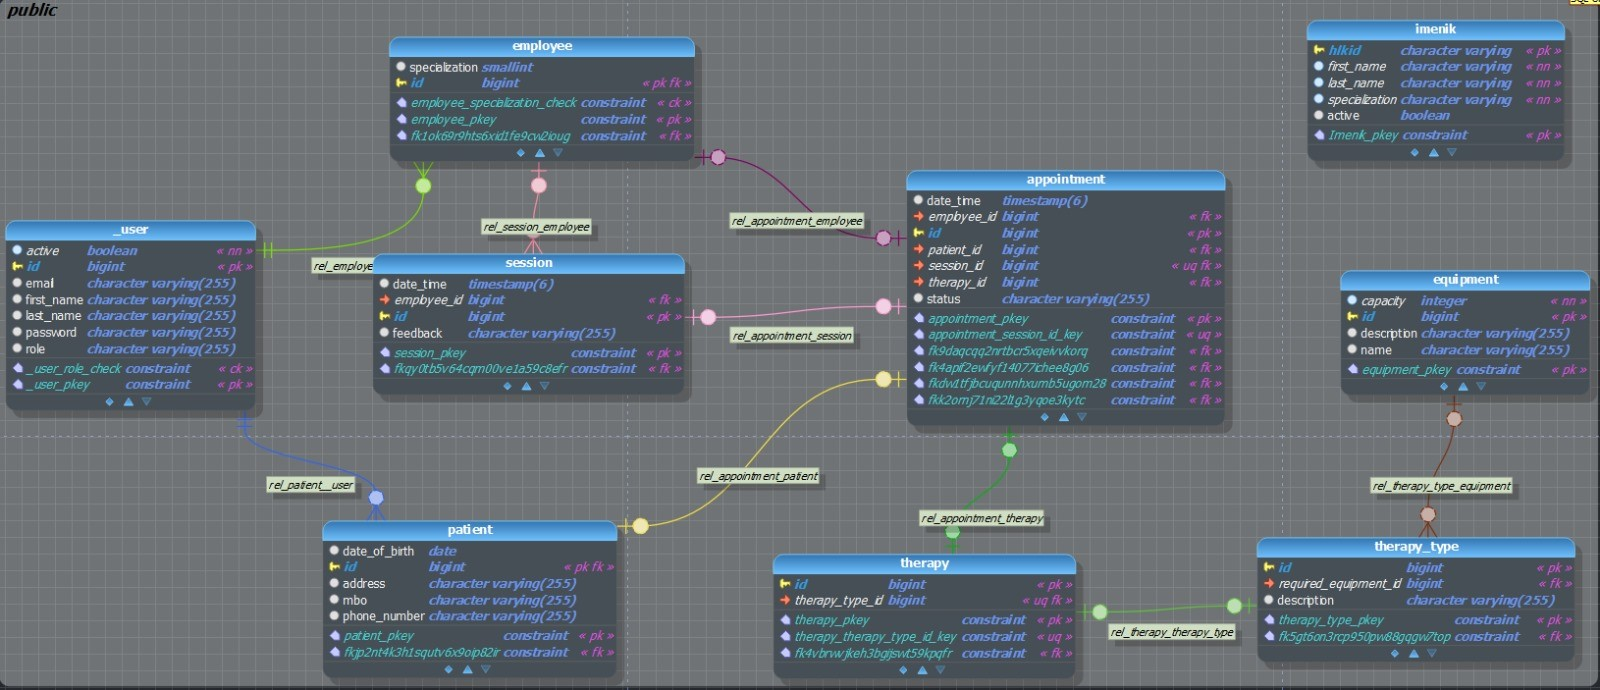
\includegraphics[width=1\linewidth]{slike/database_pr1.jpg}
			    \caption{Dijagram baze podataka}
			    
			    \label{fig:enter-label}
			\end{figure}
			\eject
			
			
		\section{Dijagram razreda}
		
			\textit{Potrebno je priložiti dijagram razreda s pripadajućim opisom. Zbog preglednosti je moguće dijagram razlomiti na više njih, ali moraju biti grupirani prema sličnim razinama apstrakcije i srodnim funkcionalnostima.}
            
            \textbf{\textit{dio 1. revizije}}
            
            \textit{Prilikom prve predaje projekta, potrebno je priložiti potpuno razrađen dijagram razreda vezan uz \textbf{generičku funkcionalnost} sustava. Ostale funkcionalnosti trebaju biti idejno razrađene u dijagramu sa sljedećim komponentama: nazivi razreda, nazivi metoda i vrste pristupa metodama (npr. javni, zaštićeni), nazivi atributa razreda, veze i odnosi između razreda.}\newline

    Backend arhitektura prikazana je u sljedećim dijagramima označenim brojevima 4.3, 4.4.
    Implementirane metode direktno komuniciraju s bazom podataka te vraćaju tražene podatke  poput popisa dijelatnika, opreme, provjere je li dijelatnik i dalje aktivan.
		   \begin{figure}[H]
    \centering
    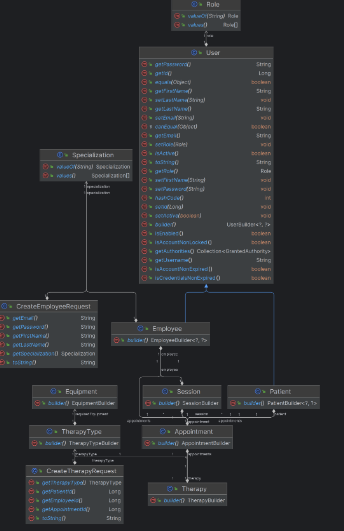
\includegraphics[width=0.46\linewidth]{slike/razredi1.png}
    \caption{Dijagram razreda}
    \label{fig:enter-label}
\end{figure}
Razredi Employee i Patient  specifikacija su razreda User pa nasljeđuju njegove public atribute i metode.
Razred Patient predstavlja model pacijenta u medicinskom sustavu. Ovaj razred proširuje osnovni razred \verb|User|, sadržavajući atribute kao što su adresa, datum rođenja, matični broj osiguranika (MBO), broj telefona te listu termina na koje je pacijent naručen.
Razred User predstavlja osnovni model korisnika u sustavu. Ovaj razred obuhvaća osnovne informacije o korisniku, uključujući ime, prezime, email adresu, lozinku i status aktivnosti korisničkog računa. Dodatno, svaki korisnik ima dodijeljenu ulogu koja se koristi za upravljanje ovlastima unutar sustava.
Razred Employee predstavlja model zaposlenika u medicinskom sustavu. Ovaj razred proširuje osnovni razred User, dodajući specifične atribute i odnose relevantne za zaposlenike u sustavu. Sadrži privatni atribut Specialization specialization koji predstavlja specijalizaciju zaposlenika, što može uključivati različite medicinske oblasti ili specifične zadatke unutar sustava.

Razred Specialization predstavlja enumeraciju koja sadrži različite vrste specijalizacija dijelatnika u medicinskom sustavu. 
Razred Session predstavlja radnu sesiju unutar medicinskog sustava. Ovaj razred omogućuje praćenje sesija između zaposlenika i pacijenata. 
Razred Equipment predstavlja opremu koja se koristi u medicinskom sustavu. Ovaj razred pruža informacije o različitim vrstama opreme, uključujući jedinstveni identifikator opreme, kapacitet, opis i naziv opreme. 
Razred Therapy predstavlja terapiju unutar medicinskog sustava. 
Razred TherapyType predstavlja vrstu terapije u sustavu. \\
\begin{figure}[H]
    \centering
    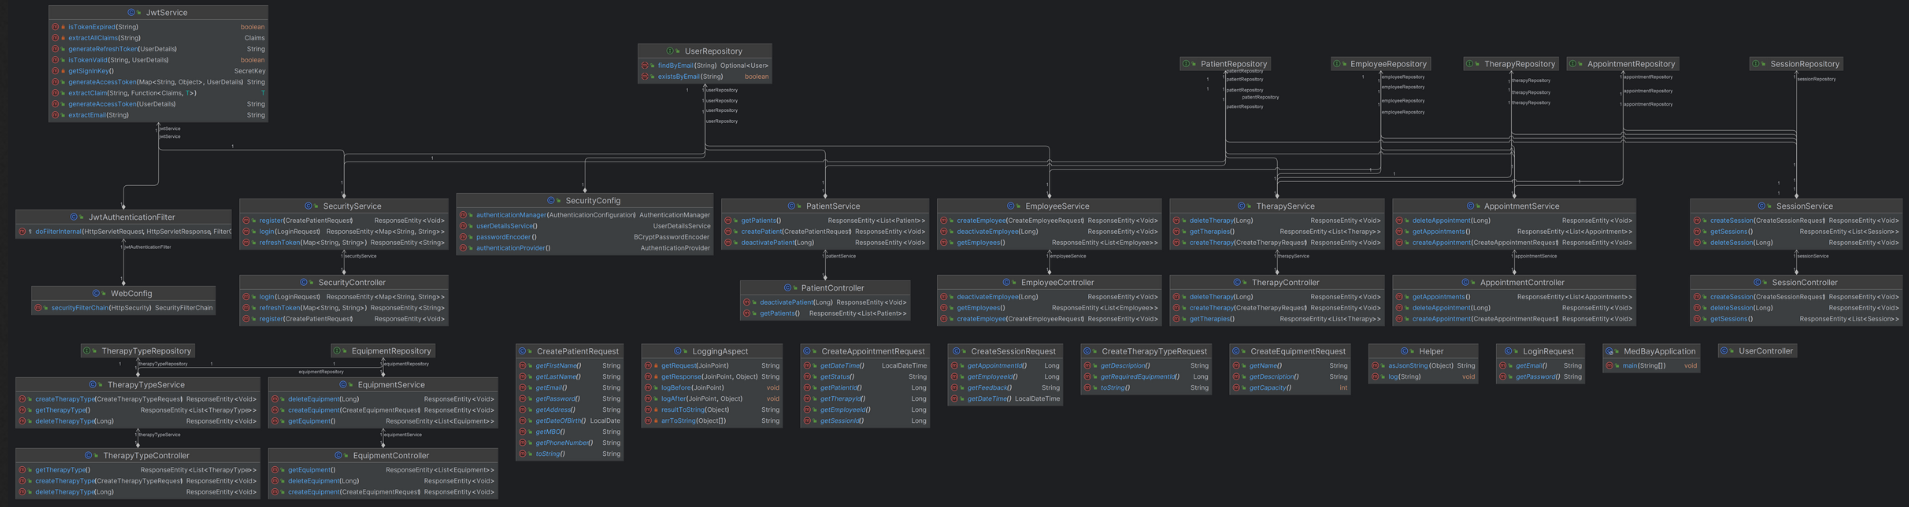
\includegraphics[width=1\linewidth]{slike/razredi2.png}
    \caption{Dijagram razreda, 2.dio}
    \label{fig:enter-label}
\end{figure}


Svaki od ovih entiteta slijedi obrazac  \verb|Controller -> Service -> Repository| za obavljanje operacija nad podacima.

Na primjer, entitet Employee posjeduje EmployeeController, EmployeeService i EmployeeRepository. Ovi razredi zajednički omogućuju upravljanje informacijama o zaposlenicima, uključujući njihovu autentikaciju. Kroz ovaj ciklus, Controller komunicira s Servisom, a Servis dalje s Repozitorijem, osiguravajući konzistentan i siguran pristup podacima.

Osim toga, entiteti poput Therapy, Appointment i Session imaju svoje setove Controllera, Servisa i Repozitorija koji omogućuju operacije vezane uz terapije, narudžbe pacijenata i sesije.

Bitna karakteristika ovog organiziranog pristupa je da Controller vraća odgovarajući HTTP status i tražene informacije (klasa, string ili ništa) u obliku JSON-a. Ovaj proces olakšava komunikaciju između različitih dijelova sustava, pružajući jasnu i strukturiranu komunikaciju među različitim slojevima aplikacije.

Kad Patient izvrši registraciju ili prijavu, procesi autentikacije i autorizacije upravljaju se putem SecurityControllera i SecurityServicea. Ovi kontroleri i servisi surađuju s SecurityConfig-om, implementiranim pomoću WebConfig, kako bi provjerili je li pacijent, administrator ili zdravstveni djelatnik autoriziran i autentificiran za svaku radnju koju žele izvršiti u sustavu.

SecurityController omogućuje upravljanje zahtjevima vezanim uz sigurnost, poput registracije i prijave korisnika, dok SecurityService sadrži logiku autentikacije i autorizacije. Ove komponente zajednički rade kako bi osigurale siguran pristup podacima i funkcionalnostima sustava.

Kroz SecurityConfig i WebConfig, postavke sigurnosti konfiguriraju se prema tipu korisnika. Ovaj postupak osigurava da pacijenti, administratori i zdravstveni djelatnici imaju odgovarajuće privilegije za izvršavanje željenih radnji, uzimajući u obzir autentikaciju i autorizaciju.

Ova struktura omogućuje efikasno i sigurno upravljanje pristupom resursima u sustavu, osiguravajući da svaki korisnik ima odgovarajuće ovlasti za obavljanje svojih funkcija u skladu s postavljenim sigurnosnim pravilima.\\

 

 

 

  

   
   \textbf{\textit{dio 2. revizije}}\\			
			
			\textit{Prilikom druge predaje projekta dijagram razreda i opisi moraju odgovarati stvarnom stanju implementacije}
			
			
			
			\eject
		
		\section{Dijagram stanja}
			
			
			\textbf{\textit{dio 2. revizije}}\\
			
			\textit{Potrebno je priložiti dijagram stanja i opisati ga. Dovoljan je jedan dijagram stanja koji prikazuje \textbf{značajan dio funkcionalnosti} sustava. Na primjer, stanja korisničkog sučelja i tijek korištenja neke ključne funkcionalnosti jesu značajan dio sustava, a registracija i prijava nisu. }
			
			
			\eject 
		
		\section{Dijagram aktivnosti}
			
			\textbf{\textit{dio 2. revizije}}\\
			
			 \textit{Potrebno je priložiti dijagram aktivnosti s pripadajućim opisom. Dijagram aktivnosti treba prikazivati značajan dio sustava.}
			
			\eject
		\section{Dijagram komponenti}
		
			\textbf{\textit{dio 2. revizije}}\\
		
			 \textit{Potrebno je priložiti dijagram komponenti s pripadajućim opisom. Dijagram komponenti treba prikazivati strukturu cijele aplikacije.}
	\chapter{Implementacija i korisničko sučelje}
		
		
		\section{Korištene tehnologije i alati}
	
			
\textbf{	KORIŠTENE TEHNOLOGIJE
} 

Prilikom izrade web aplikacija za upravljanje rehabilitacijom koristili smo razne tehnologije kako bismo pružili korisnicima učinkovit i interaktivan doživljaj. \textit{Backend} aplikacije razvili smo koristeći \href{https://www.spring.io/projects/spring-boot}{Spring Boot}, \href{https://www.oracle.com/java}{Java} bazirani okvir, koji omogućava brz i jednostavan razvoj logike sa serverske strane. \href{https://www.oracle.com/java}{Java} doprinosi robustnosti i skalabilnosti našeg \textit{backend} sustava.

Za dinamičke i interaktivne elemente na korisničkom sučelju, koristili smo \href{https://www.developer.mozilla.org/en-US/docs/Web/JavaScript}{JavaScript}, dok je \href{https://www.reactjs.org}{React}, popularni \href{https://www.developer.mozilla.org/en-US/docs/Web/JavaScript}{JavaScript} okvir, omogućio izgradnju efikasnog korisničkog sučelja. \href{https://www.reactjs.org}{React}, koristeći koncept komponenti, pojednostavljuje organizaciju i održavanje koda, pridonoseći poboljšanju korisničkog iskustva i olakšavajući upravljanje stanjem naše aplikacije.

Podaci o pacijentima, terapijama i terminima pohranjeni su u \href{https://www.postgresql.org}{PostgreSQL} bazi podataka koja pruža pouzdanu podršku. \href{https://www.postgresql.org}{PostgreSQL}, kao snažan objektno-relacijski sustav upravljanja bazama podataka, omogućava nam efikasno upravljanje informacijama uz podršku za kompleksne upite i transakcije. Osim toga, \href{https://www.developer.mozilla.org/en-US/docs/Web/HTML}{HTML} i \href{https://www.developer.mozilla.org/en-US/docs/Web/CSS}{CSS} koriste se za strukturiranje sadržaja web stranice i stilizaciju, stvarajući tako funkcionalno i atraktivno korisničko sučelje.

Dokumentacija projekta oblikovana je pomoću \href{https://www.overleaf.com/learn/latex/Learn_LaTeX_in_30_minutes}{LaTeX} sustava za pripremu dokumenata, pružajući precizno formatiranje i organizaciju. Za organizaciju sastanaka i suradnju koristili smo \href{https://www.markdownguide.org}{Markdown} format, pružajući jednostavan i čitljiv način za pisanje i dijeljenje informacija.

U procesu zajedničkog rada, pisanja koda i praćenja promjena koristili smo \href{https://git-scm.com/}{Git}. Omogućavao je stvaranje, pregledavanje i spajanje promjena koda, čime se postizavao učinkovit timski rad. Sve ove tehnologije integrirane su u našem projektu kako bismo osigurali da interakcija između bolesnika, djelatnika zdravstvene ustanove i administratora bude glatka, učinkovita i prilagođena specifičnim ulogama i funkcionalnim zahtjevima svakog dionika.

\href{https://www.python.org/}{Python} je bio ključan u razvoju našeg AI chat bota, iskoristili smo njegove sposobnosti u strojnom učenju i obradi prirodnog jezika za stvaranje interaktivnog i inteligentnog sučelja za korisnike. \href{https://www.python.org/}{Python} smo još koristili u kombinaciji sa \href{https://www.selenium.dev/documentation/webdriver/}{Selenium WebDriverom} za automatizaciju testiranja korisničkog sučelja, omogućavajući simulaciju stvarnih interakcija korisnika i osiguravajući pouzdanost naše web aplikacije.

\textbf{KORIŠTENI ALATI
}

U procesu razvoja naše aplikacije koristili smo raznovrsne alate kako bismo unaprijedili različite aspekte projekta. Alat \href{https://www.heroku.com}{Heroku}, poznat po svojoj \textit{cloud} platformi, omogućio nam je jednostavno postavljanje, skaliranje i učinkovito upravljanje web aplikacijama. Korištenjem \href{https://www.heroku.com}{Heroku}-a, značajno smo pojednostavili proces implementacije i održavanja naše aplikacije.

Za potrebe pisanja, testiranja i ispravljanja koda koristili smo \href{https://www.visualstudio.com}{Visual Studio Code} (\href{https://www.visualstudio.com}{VSCode}), integrirano razvojno okruženje (IDE). \href{https://www.visualstudio.com}{VSCode} pružio je alate koji su povećali efikasnost našeg tima tijekom razvoja aplikacije. \href{https://www.jetbrains.com/idea}{IntelliJ IDEA}, kao razvojno okruženje specifično za Java programski jezik, optimizirao je rad na \textit{backend} dijelu naše aplikacije. 

\href{https://github.com}{GitHub}, platforma za upravljanje verzijama koda i suradnju timova, poslužila nam je za praćenje promjena, upravljanje zadacima te implementaciju \textit{pull requestova}, unapređujući suradnju tima. Za brzu i jednostavnu komunikaciju te video razgovore koristili smo \href{https://discord.com}{Discord}, pružajući središnje mjesto za razmjenu informacija između članova tima.


\href{https://www.notion.so}{Notion}, kao alat za organizaciju zadataka, vođenje bilješki sastanaka i općenito upravljanje projektom, korišten je kako bi pridonio boljoj organizaciji i praćenju napretka. \href{https://www.overleaf.com}{Overleaf}, online platforma za suradničko pisanje dokumenata u LaTeX formatu, olakšala je stvaranje i uređivanje dokumentacije našeg projekta.
\href{https://www.visual-paradigm.com}{Visual Paradigm} pruža alate za izradu različitih dijagrama, a mi smo ga koristili za izradu dijagrama obrasca uporabe, sekvencijskih dijagrama, dijagrama stanja, aktivnosti i komponenata potrebnih za dokumentaciju. 

\href{https://www.figma.com}{Figma}, alat za dizajn, poslužio nam je u izradi vizualnih planova naše web aplikacije. Kroz Figmu definirali smo izgled \textit{frontend} dijela naše aplikacije. \href{https://www.adobe.com/products/premiere.html}{Adobe Premiere Pro} i \href{https://www.adobe.com/products/audition.html}{Audition} koristili smo za video i audio produkciju, stvarajući marketinške materijale i prezentacije vezane uz našu aplikaciju.

Naša interakcija s \href{https://openai.com/gpt}{ChatGPT}om bila je višestruko korisna, pružajući podršku u različitim aspektima, uključujući punjenje baze podataka te pružanje informacija i savjeta za vrijeme razvoja projekta. 


 		Napomena: Prilikom klika u tekstu na nazive korištenih alata i tehnologija otvara se internet poveznica na kojoj se može saznati više informacija o njima. 
		Unatoč tome ovdje su navedene internet poveznice na kojima je moguće saznati više:  
		https://www.spring.io/projects/spring-boot, \newline https://www.oracle.com/java,  
		https://www.developer.mozilla.org/en-US/docs/Web/JavaScript, 
		https://www.reactjs.org, https://www.postgresql.org, 
		\newline https://www.developer.mozilla.org/en-US/docs/Web/HTML,
		\newline https://www.developer.mozilla.org/en-US/docs/Web/CSS, 
		\newline https://www.overleaf.com/learn/latex,  
		\newline https://www.markdownguide.org, https://git-scm.com, 
		https://www.heroku.com, https://www.visualstudio.com, 
		\newline https://www.jetbrains.com/idea, https://github.com, 
		\newline https://discord.com, https://www.notion.so, 
		https://www.overleaf.com, 
		\newline https://www.visual-paradigm.com, https://www.figma.com, 
		\newline https://www.adobe.com/products/premiere.html, 
		\newline https://www.adobe.com/products/audition.html, 
		\newline https://openai.com/gpt, https://www.python.org/,
		\newline https://www.selenium.dev/documentation/webdriver/

			\eject 
		
	
			\section{Ispitivanje programskog rješenja}
			
			Ispitivanje komponenti provedeno je na razredima  \href{https://github.com/Project-MedBay/backend/blob/main/src/test/java/com/medbay/TherapyTypeServiceTest.java}{TherapyTypeService} 
			i \href{https://github.com/Project-MedBay/backend/blob/main/src/test/java/com/medbay/TherapyServiceTest.java}{TherapyService} u okruženju \texttt{com.medbay}. Slijede rezultati pojedinih ispitnih slučajeva:
			\newline \textbf{Rezultati ispitivanja komponenti za \href{https://github.com/Project-MedBay/backend/blob/main/src/test/java/com/medbay/TherapyTypeServiceTest.java}{TherapyTypeService}}

			\begin{enumerate}
				\item \textbf{Test: getTherapyType\_ReturnsListOfTherapyTypes}
				\begin{itemize}
					\item \textit{Opis:} Provjera vraćanja liste tipova terapija.
					\item \textit{Rezultat:} Test uspješan. Vraćena lista tipova terapija.
				\end{itemize}
\begin{lstlisting}[language=Java]
@Test
void getTherapyType_ReturnsListOfTherapyTypes() {
	List<TherapyType> expectedTherapyTypes = Arrays.asList(buildTherapyType("1"), buildTherapyType("2"));
	when(therapyTypeRepository.findAll()).thenReturn(expectedTherapyTypes);
	ResponseEntity<List<TherapyType>> response = therapyTypeService.getTherapyType();
	assertEquals(HttpStatus.OK, response.getStatusCode());
	assertEquals(expectedTherapyTypes, response.getBody());
	}
\end{lstlisting}

				\item \textbf{Test: getTherapyType\_WhenNoTherapyTypes\_ReturnsEmptyList}
				\begin{itemize}
					\item \textit{Opis:} Provjera vraćanja prazne liste kada nema tipova terapija.
					\item \textit{Rezultat:} Test uspješan. Vraćena prazna lista.
				\end{itemize}
\begin{lstlisting}[language=Java]
@Test
void getTherapyType_WhenNoTherapyTypes_ReturnsEmptyList() {
	when(therapyTypeRepository.findAll()).thenReturn(Collections.emptyList());
	ResponseEntity<List<TherapyType>> response = therapyTypeService.getTherapyType();
	assertEquals(HttpStatus.OK, response.getStatusCode());
	assertTrue(Objects.requireNonNull(response.getBody()).isEmpty());
		}
\end{lstlisting}

				\item \textbf{Test: getTherapyType\_WhenRepositoryThrowsException\_ReturnsErrorResponse}
				\begin{itemize}
					\item \textit{Opis:} Provjera odziva na iznimku iz repozitorija.
					\item \textit{Rezultat:} Test uspješan. Izazvana iznimka.
				\end{itemize}

\begin{lstlisting}[language=Java]
@Test
void getTherapyType_WhenRepositoryThrowsException_ReturnsErrorResponse() {
	when(therapyTypeRepository.findAll()).thenThrow(new RuntimeException("Database error"));
	assertThrows(RuntimeException.class, () -> therapyTypeService.getTherapyType());
}
\end{lstlisting}
			\end{enumerate}
			
			Svi ispitni slučajevi su prošli uspješno, što ukazuje na pouzdanost i stabilnost implementiranih funkcionalnosti u razredu \texttt{TherapyTypeService}. 
			\begin{figure}[h]
				\centering
				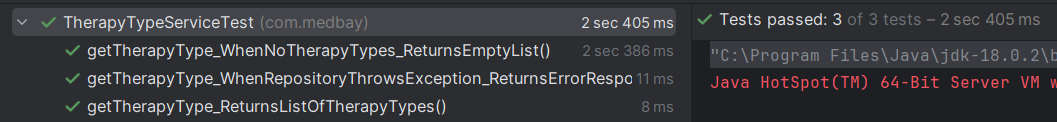
\includegraphics[width=1\linewidth]{slike/therapyTypeServiceTest.png}
				\caption{Rezultati testova za TherapyTypeService}
				\label{fig:enter-label}
			\end{figure}

			\newblock \textbf{Rezultati ispitivanja komponenti za \href{https://github.com/Project-MedBay/backend/blob/main/src/test/java/com/medbay/TherapyServiceTest.java}{TherapyService}}

			\begin{enumerate}
				\item \textbf{Test: getTherapies\_ReturnsListOfTherapies}
				\begin{itemize}
					\item \textit{Opis:} Provjera vraćanja liste terapija.
					\item \textit{Rezultat:} Test uspješan. Vraćena lista terapija.
				\end{itemize}
\begin{lstlisting}[language=Java]
@Test
void getTherapies_ReturnsListOfTherapies() {
	List<Therapy> expectedTherapies = Arrays.asList(buildTherapy("1"), buildTherapy("2"));
	when(therapyRepository.findAll()).thenReturn(expectedTherapies);
	ResponseEntity<List<Therapy>> response = therapyService.getTherapies();
	assertEquals(HttpStatus.OK, response.getStatusCode());
	assertEquals(expectedTherapies, response.getBody());
}
\end{lstlisting}
					
				\item \textbf{Test: getTherapies\_WhenNoTherapies\_ReturnsEmptyList}
				\begin{itemize}
					\item \textit{Opis:} Provjera vraćanja prazne liste kada nema terapija.
					\item \textit{Rezultat:} Test uspješan. Vraćena prazna lista.
				\end{itemize}

\begin{lstlisting}[language=Java]
@Test
void getTherapies_WhenNoTherapies_ReturnsEmptyList() {
	when(therapyRepository.findAll()).thenReturn(Collections.emptyList());
	ResponseEntity<List<Therapy>> response = therapyService.getTherapies();
	assertEquals(HttpStatus.OK, response.StatusCode());
	assertTrue(Objects.requireNonNull(response.getBody()).isEmpty());
}
\end{lstlisting}
					
				\item \textbf{Test: deleteTherapy\_WhenTherapyExists\_DeletesTherapy}
				\begin{itemize}
					\item \textit{Opis:} Provjera brisanja postojeće terapije.
					\item \textit{Rezultat:} Test uspješan. Terapija izbrisana.
				\end{itemize}

\begin{lstlisting}[language=Java]
@Test
void deleteTherapy_WhenTherapyExists_DeletesTherapy() {
	Long therapyId = 1L;
	when(therapyRepository.existsById(therapyId)).thenReturn(true);
	ResponseEntity<Void> response = therapyService.deleteTherapy(therapyId);
	assertEquals(HttpStatus.OK, response.getStatusCode());
	verify(therapyRepository).deleteById(therapyId);
}
\end{lstlisting}
					
				\item \textbf{Test: deleteTherapy\_WhenTherapyDoesNotExist\_ReturnsNotFound}
				\begin{itemize}
					\item \textit{Opis:} Provjera odziva kada terapija ne postoji.
					\item \textit{Rezultat:} Test uspješan. Vraćen status "Nije pronađeno".
				\end{itemize}

\begin{lstlisting}[language=Java]
@Test
void deleteTherapy_WhenTherapyDoesNotExist_ReturnsNotFound() {
	Long therapyId = 1L;
	when(therapyRepository.existsById(therapyId)).thenReturn(false);
	ResponseEntity<Void> response = therapyService.deleteTherapy(therapyId);
	assertEquals(HttpStatus.NOT_FOUND, response.getStatusCode());
	verify(therapyRepository, never()).deleteById(therapyId);
}
\end{lstlisting}
					
			\end{enumerate}
			\begin{figure}[!h]
				\centering
				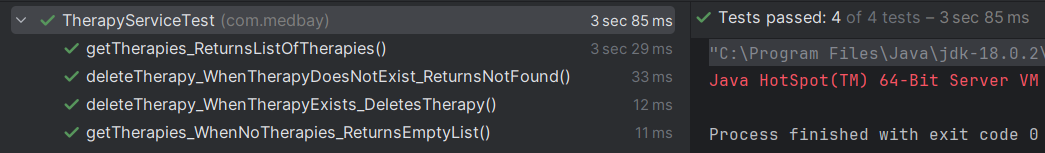
\includegraphics[width=1\linewidth]{slike/therapyServiceTest.png}
				\caption{Rezultati testova za TherapyService}
				\label{fig:enter-label}
			\end{figure}


			Svi testovi su uspješno prošli, što ukazuje na pouzdanost i ispravnost implementacije u razredu \texttt{TherapyService}. \newline

			Napomena: Prilikom klika na naziv razreda korištenih za testiranje otvara se internet poveznica na kojoj se može vidjeti izvorni kod testova.

			
			
			\subsection{Ispitivanje sustava}
			Svi testovi osim registracije i zaboravljene lozinke izvršeni su uz pomoć Selenium WebDrivera . Ispitivanje se radilo po obrascima uporabe kako bi
se provjerile funkcionalnosti sustava. Prikazivanje ispitivanja UC1, UC3, UC4, UC5, UC6 i UC13 (uključujući UC7).
			\newline
			\textbf{Ispitni sučaj 1: Registracija} 
			\begin{enumerate}
				\item Otvaranje stranice za registraciju.
				\item Unos obveznih podataka: ime, prezime, email, datum rođenja, adresa, broj telefona, MBO, lozinka.
				\item Riješavanje Google reCAPTCHA.
				\item Klik na gumb za registraciju.
			\end{enumerate}
			\textbf{Očekivani izlaz:}
			\begin{enumerate}
				\item Prikaz poruke o uspjehu slanja zahtjeva za registraciju.
			\end{enumerate}
			\textbf{Rezultat:} Očekivani rezultat je zadovoljen. \color{green} Aplikacija je prošla test. \color{black} \newline
			\textbf{Ispitni sučaj 2: Prijava na stranicu} 
			\textbf{Ulaz:}
			\begin{enumerate}
				\item Otvaranje početne stranice.
				\item Unos e-maila i lozinka.
				\item Klik na gumb za prijavu.
			\end{enumerate}
			\textbf{Očekivani izlaz:}
			\begin{enumerate}
				\item Uspješna prijava i preusmjeravanje na početnu stranicu za pacijente.
			\end{enumerate}
			\textbf{Rezultat:} Očekivani rezultat je zadovoljen. \color{green} Aplikacija je prošla test. \color{black} \newline
			\textbf{Ispitni slučaj 3: Promjena termina terapije}
			\begin{enumerate}
				\item Klik na prvi termin terapije.
				\item Klik na opciju "Odgodi termin".
				\item Promjena datuma termina iza posljednjeg termina terapije.
				\item Potvrda odabira i klik na gumb za potvrdu odgode.
				\item Klik na poslijednji termin terapije.
				\item Klik na opciju "Odgodi termin".
				\item Promjena datuma termina na orginalni datum.
				\item Potvrda odabira i klik na gumb za potvrdu odgode.
			\end{enumerate}
			\textbf{Očekivani izlaz:}
			\begin{enumerate}
				\item[1.a] Uspješna promjena datuma termina.
				\item[1.b] Informacije o terminu promijenjene i odgovaraju novom datumu.
				\item[2.a] Uspješna promjena datuma termina.
				\item[2.b] Informacije o terminu promijenjene i odgovaraju novom datumu.
			\end{enumerate}
			\textbf{Rezultat:} Očekivani rezultat [2.b] nije zadovoljen jer se redni broj termina prikazuje kao posljednji umjesto kao prvi, iako je u kalendaru na točnoj poziciji. Ostala očekivanja su zadovoljena. \color{red} Aplikacija nije prošla test. \color{black} \newline
			\textbf{Ispitni slučaj 4: Stvaranje novog zahtjeva za terapiju}
			\begin{enumerate}
				\item Klik na opciju "Nova terapija".
				\item Odabir vrste terapije i unos potrebnih datuma.
				\item Unos verifikacijski podataka terapije sa uputnice.
				\item Potvrda odabira i klik na gumb za završetak.
				\item Prikaz poruke o uspješnom zahtjevu za novu terapiju.
			\end{enumerate}
			\textbf{Očekivani izlaz:}
			\begin{enumerate}
				\item Uspješno stvaranje terapije i prikaz potvrde. 
				\item Dodavanje termina u raspored korisnika.
			\end{enumerate}
			\textbf{Rezultat:} Sva očekivanja su zadovoljena. \color{green} Aplikacija je prošla test. \color{black} \newline
			\textbf{Ispitni slučaj 5: Zaboravljena lozinka}
			\begin{enumerate}
				\item Otvaranje početne stranice.
				\item Klik na "Zaboravljena lozinka".
				\item Upis e-mail adrese za oporavak lozinke.
				\item Klik na poveznicu koja je došla e-mailom.
				\item Upis i potvrda nove lozinke.
				\item Klik na gumb "Reset password".
				\item Spremanje promjena.
			\end{enumerate}
			\textbf{Očekivani izlaz:}
			\begin{enumerate}
				\item Sustav šalje elektronsku poštu s obrascem za promjenu lozinke.
				\item Nakon ispunjavanja obrasca uspješno promijenjena lozinka.
			\end{enumerate}
			\textbf{Rezultat:} Sva očekivanja su zadovoljena. \color{green} Aplikacija je prošla test. \color{black} \newline
			\textbf{Ispitni slučaj 6: Promjena bilješke o terminu pacijenta}
			\begin{enumerate}
				\item Odabir termina kojem želimo promijeniti bilješku o terminu.
				\item Klik na "Uredi".
				\item Promjena bilješke o terminu.
				\item Spremanje promjena.
			\end{enumerate}
			\textbf{Očekivani izlaz:}
			\begin{enumerate}
				\item Ažuriranje bilješke o terminu.
			\end{enumerate}
			\textbf{Rezultat:} Očekivani rezultat je ostvaren. \color{green} Aplikacija je prošla test. \color{black} \newline

			
			\eject 
		
		
		\section{Dijagram razmještaja}
						
			Dijagram razmještaja opisuje topologiju sustava, fizičku arhitekturu i razmještaj programskih sustava te kako te cjeline komuniciraju. Na dijagramu imamo dva glavna čvora. Prvo imamo uređaj korisnika (PC, mobitel) preko čijeg web preglednika korisnik putem HTTPS-a dohvaća informacije iz drugog čvora, mjesta gdje je pohranjen kod aplikacije, baza podataka i gdje je upogonjena aplikacija. Riječ je o Herokuu, platformi za pogonjenje aplikacija na oblaku. Heroku funkcionira pomoću \textit{dynoa}, fleksibilnih i izoliranih kontejnera koji sadrže Linux. Naša web aplikacija koristi tri \textit{dynoa}. Na prvome se nalazi frontend dio aplikacije koji je napisan u okviru React. Druga komponenta je kontejner na kojemu se sadrži \textit{backend} dio aplikacije. Tu je najbitnija Spring aplikacija koja reagira na zahtjeve \textit{frontenda} i komunicira s bazom podataka, a prisutan je i kratki kod koji omogućuje rad AI bota na našoj aplikaciji. Tu se još nalazi i zadnji \textit{dyno}, Herokuova PostgreSQL usluga gdje se nalazi baza podataka koju aplikacija koristi. Kontejneri za \textit{frontend} i \textit{backend} komuniciraju HTTPS protokolom, a \textit{backend} i baza podataka s protokolima koje osmišlja i definira sam Heroku.

            \begin{figure}[H]
             \centering
             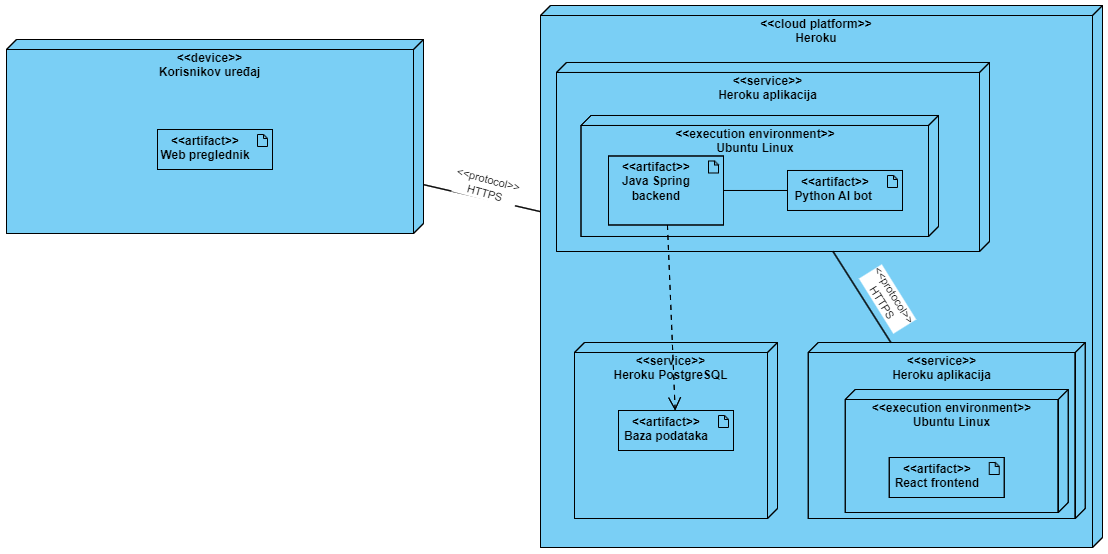
\includegraphics[width=1\linewidth]{slike/Dijagram razmjestaja.png}
             \caption{Dijagram razmještaja}
             \end{figure}
			\eject
		
		\section{Upute za puštanje u pogon}
		
		
U postavljanju i puštanju u pogon naše aplikacije ključnu ulogu igra Heroku CLI (Command Line Interface), moćan naredbeni alat koji pojednostavljuje interakciju s Heroku platformom izravno iz terminala. Instalirali smo Heroku CLI na lokalnom računalu kako bismo iskoristili njegove funkcionalnosti za upravljanje aplikacijama na Heroku platformi.

Naša integrirana strategija razvoja i puštanja u pogon koristi niz ključnih značajki Heroku platforme:

1. Automatsko puštanje u pogon s GitHub-a:
\newline- GitHub repozitorij povezan je s Heroku, omogućujući jednostavano automatsko puštanje u pogon naše aplikacije.
\newline- Svaka promjena na glavnoj grani GitHuba automatski pokreće puštanje u pogon na Heroku platformi.

2. Konfiguracijske Datoteke na Heroku:
\newline- Heroku nam omogućava preciznu konfiguraciju putem posebnih datoteka koje definiraju okruženje za našu aplikaciju.
\newline- Detaljno smo definirali parametre poput verzija jezika (Java, Python) i aktivnih profila za Spring.

3. Korištenje Financijske Potpore od Heroku:
\newline- Naša organizacija prima financijsku potporu od Heroku platforme, pružajući nam sredstva za korištenje resursa.


4. Baza Podataka na Heroku:
\newline- Integrirali smo Heroku Postgres "add-on" za potrebe baze podataka.
\newline- Heroku Postgres pruža siguran pristup bazama podataka putem pridruženih akreditiva.
   \begin{figure}[H]
       \centering
       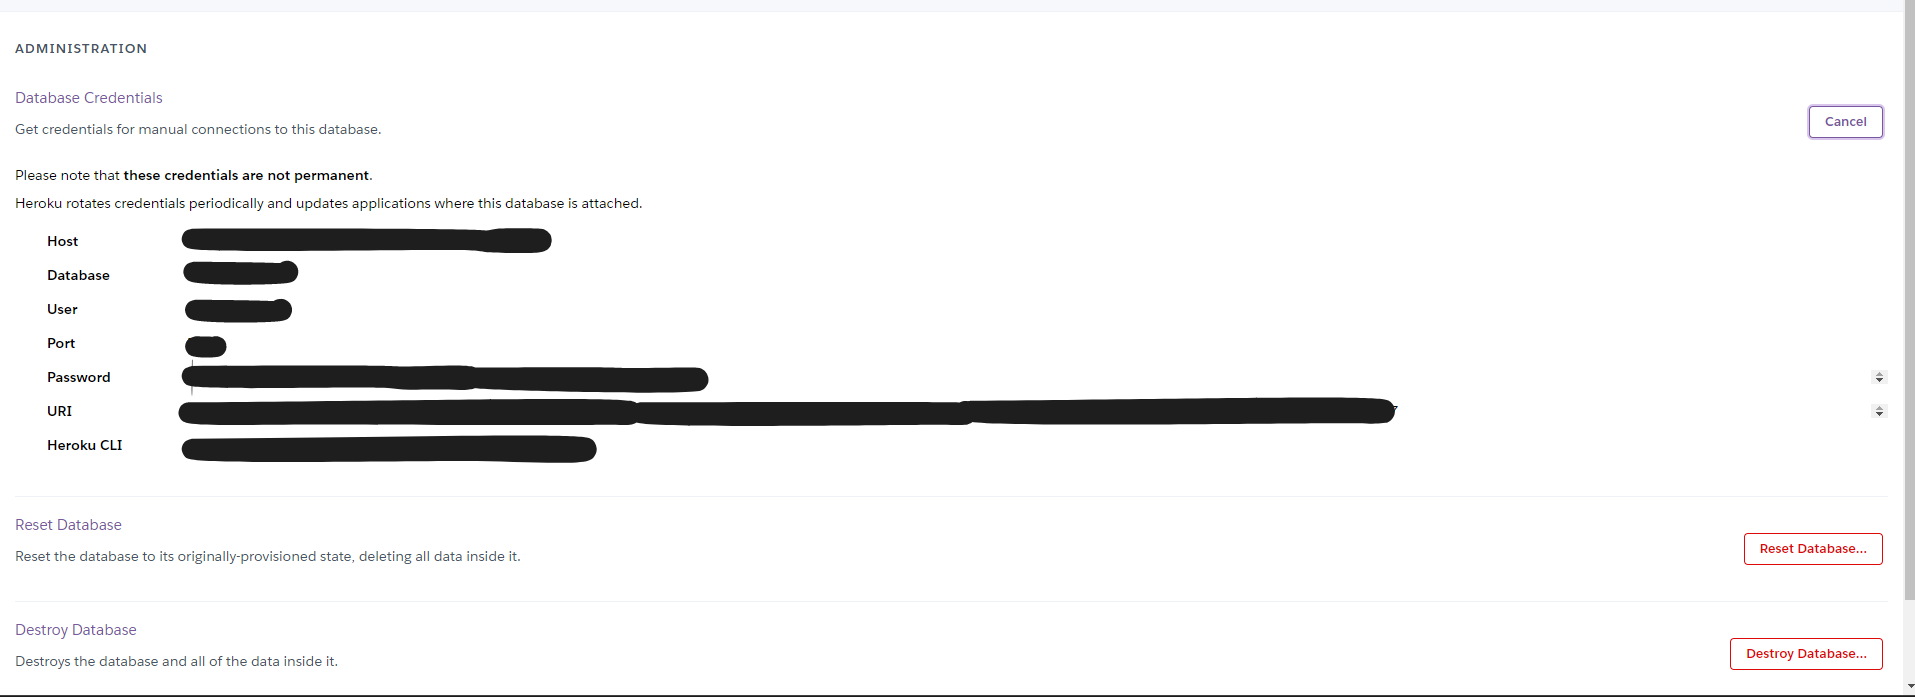
\includegraphics[width=1\linewidth]{slike/credentials.png}
       \caption{Akreditivi za našu aplikaciju}
       \label{fig:enter-label}
   \end{figure}

5. Dinamičko Okruženje s  dinamičkim kontejnerima:
\newline- Korištenjem dinamičkih kontejnera na Heroku stvaramo virtualno okruženje koje omogućuje izvršavanje i hostanje naše aplikacije.
\newline- Ime domene "medbay.life" registrirano je putem "Namecheap"-a, dok smo HTTPS certifikat dobili kroz Cloudflare za sigurnu komunikaciju.

6. Praćenje i evidentiranje:
\newline- Heroku pruža napredne alate za praćenje performansi, uključujući detaljne evidencije za svaki zahtjev poslan aplikaciji.
\newline- Metrike i analize omogućuju nam praćenje ponašanja aplikacije u stvarnom vremenu.
   \begin{figure}[H]
       \centering
       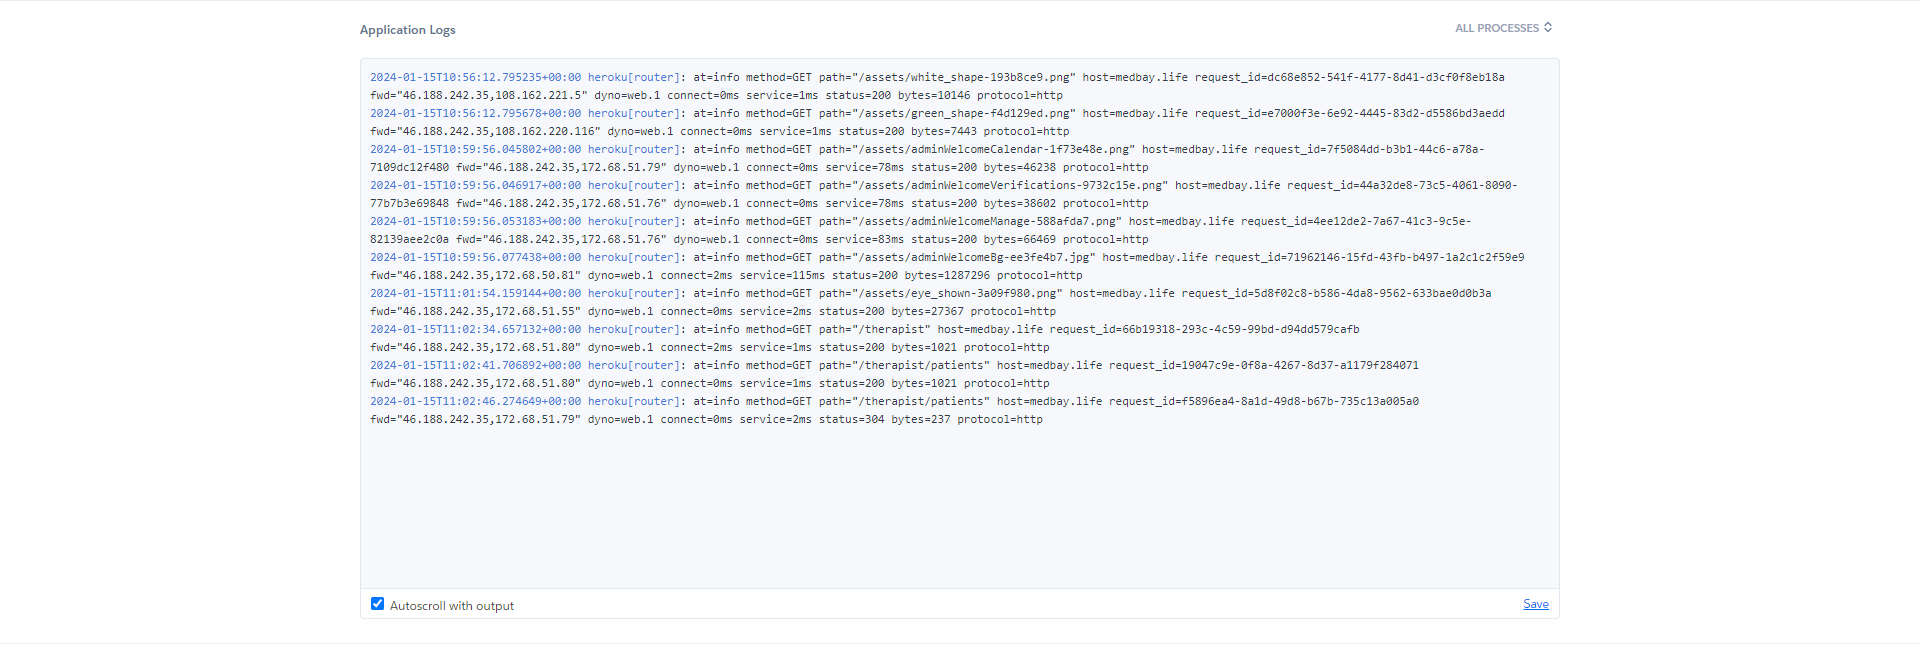
\includegraphics[width=1\linewidth]{slike/appLogs.png}
       \caption{Aplikacijsko evidentiranje}
       \label{fig:enter-label}
   \end{figure}


\begin{figure}[H]
    \centering
    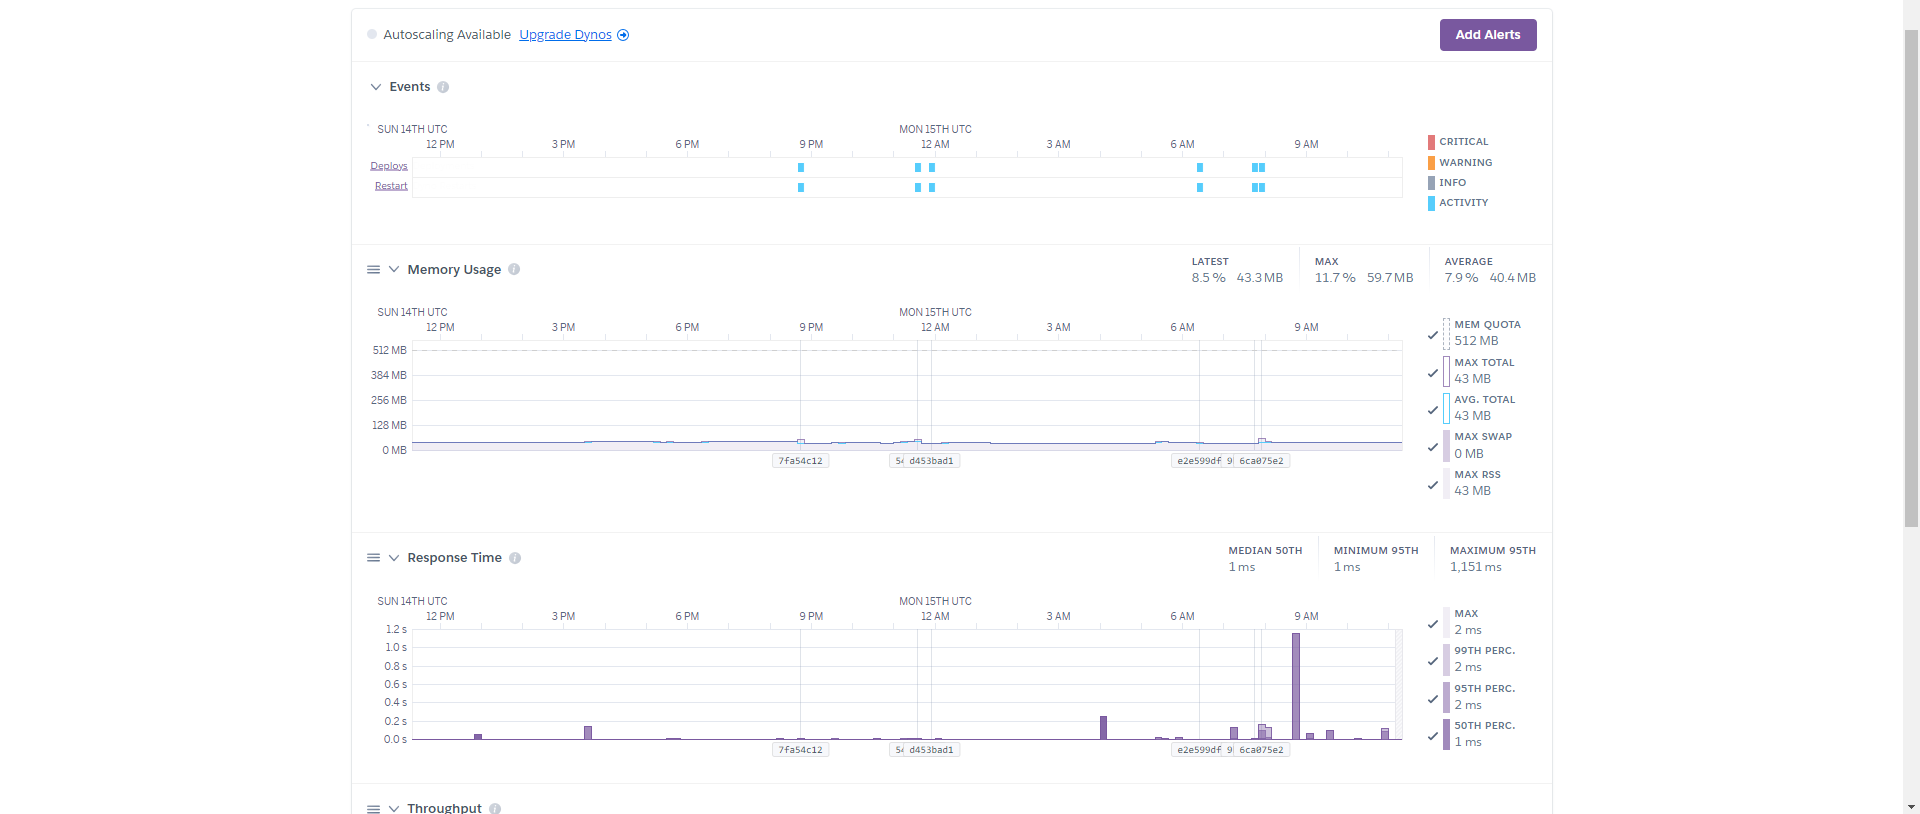
\includegraphics[width=1\linewidth]{slike/metrics.png}
    \caption{Metrika aplikacija}
    \label{fig:enter-label}
\end{figure}
7. Paketi za izgradnju:
\newline- Integrirali smo različite Pakete za izgradnju prilagođene jezicima koje koristimo (npr., Python, Java).
\newline- Automatski konfiguriraju okolinu i podržavaju različite jezične specifikacije.

Ovaj sveobuhvatan pristup omogućava nam efikasan ciklus razvoja i puštanja u pogon aplikacije. Kombinacijom GitHuba, Heroku platforme, i alata poput Heroku CLI-a, postižemo stabilan i automatski proces implementacije koji podržava dinamično okruženje naše aplikacije.


\textbf{Općenito o načinu korištenja Heroku CLI (Command Line Interface):}

1. Instalacija Heroku CLI:
   Heroku CLI smo instalirali na lokalnom računalu, omogućujući nam jednostavan pristup naredbama i funkcionalnostima koje pruža. Za instalaciju, slijedili smo upute dostupne na [službenoj Heroku stranici za instalaciju CLI-a](https://devcenter.heroku.com/articles/heroku-cli).

2. Povezivanje s Heroku Računom:
    Pomoću Heroku CLI-a uspostavili smo vezu s našim Heroku računom, omogućavajući autentikaciju i autorizaciju za izvršavanje različitih operacija. Ova faza je ključna za pristup resursima i upravljanje aplikacijom.

3. Korištenje CLI-a za puštanje u pogon aplikacije:
    Heroku CLI smo aktivno koristili za inicijalizaciju puštanje u pogon naših aplikacija. Naredbe poput `git push heroku main` omogućuju nam jednostavano i automatsko puštanje u pogon na Heroku platformu.

4. Upotreba CLI-a za Konfiguraciju Aplikacije:
    Heroku CLI pruža alate za konfiguraciju različitih aspekata aplikacije. Kroz naredbe poput `heroku config:set` postavljali smo i mijenjali okružne varijable te druge konfiguracijske postavke prema potrebama naše aplikacije.

5. Praćenje evidencija i Performansi:
    Za praćenje evidencija i performansi aplikacije koristili smo Heroku CLI. Naredbe poput `heroku logs` omogućuju nam pregled događaja u stvarnom vremenu, pružajući važne informacije o ponašanju aplikacije.

6. Dodatne Naredbe za Upravljanje Resursima:
    Heroku CLI pruža širok spektar dodatnih naredbi za upravljanje resursima. Skaliranje aplikacije, upravljanje "add-on"-ima i druge operacije mogu se jednostavno izvršiti putem ovog sučelja.

Heroku CLI je postao ključan alat u našem procesu razvoja i deploya. Omogućuje nam jednostavnu interakciju s Heroku platformom direktno iz terminala, čime poboljšavamo produktivnost i imamo veću kontrolu nad našim aplikacijama. 


	\chapter{Zaključak i budući rad}
		
		\textbf{\textit{dio 2. revizije}}\\
		
		 \textit{U ovom poglavlju potrebno je napisati osvrt na vrijeme izrade projektnog zadatka, koji su tehnički izazovi prepoznati, jesu li riješeni ili kako bi mogli biti riješeni, koja su znanja stečena pri izradi projekta, koja bi znanja bila posebno potrebna za brže i kvalitetnije ostvarenje projekta i koje bi bile perspektive za nastavak rada u projektnoj grupi.}
		
		 \textit{Potrebno je točno popisati funkcionalnosti koje nisu implementirane u ostvarenoj aplikaciji.}
		

  Projektni zadatak bio je usmjeren na razvoj web aplikacije za praćenje i upravljanje procesima medicinske rehabilitacije, obuhvaćajući vremenski period od 23. listopada 2023. do 19. siječnja 2024. godine. Redovito smo održavali tjedne sastanke i konzultacije tijekom cijelog trajanja projekta kako bismo pratili napredak i usklađivali aktivnosti. Na početku svakog sastanka članovi tima iznosili su svoja postignuća iz prethodnog tjedna, dok smo na kraju sastanka planirali zadatke za sljedeći tjedan.

Prvu fazu projekta obilježila je podjela tima na \textit{frontend} i \textit{backend} skupine. U prvom tjednu posvetili smo se učenju Spring Boota i Reacta, ovisno o odabranoj skupini. Studenti koji nisu bili upoznati s Gitom ili GitHubom prošli su odgovarajuće vježbe. Nakon stjecanja temeljnog znanja, fokusirali smo se na razvoj ideja i mogućnosti aplikacije te definiranje funkcionalnih zahtjeva.

Suradnja unutar tima bila je ključna u oblikovanju funkcionalnosti aplikacije. Veći dio tima posvetili smo i dokumentaciji kako bismo je temeljito pripremili. Prvi izazov dogodio se sredinom studenog kada smo naišli na problem na GitHubu vezan uz nepravilno usklađivanje sekundarnih grana s glavnom granom. Sekundarne grane već su imale dodatne funkcionalnosti, ali su bile u zaostatku u odnosu na glavnu granu. Nakon uspješnog rješavanja problema, unaprijedili smo svoje vještine u radu s Gitom.

\textit{Frontend} tim koristio je alat Figma za oblikovanje izgleda aplikacije, dok se \textit{backend} tim usredotočio na implementaciju registracije, prijave i povezivanje s bazom podataka. \textit{Frontend} tim uspješno je izvršio implementaciju svog dijela koristeći React, pridonoseći ciljevima za prvu predaju projekta. Zadaci vezani uz dokumentaciju bili su raspoređeni prema kraju prve faze, gdje smo izradili dijagrame poput obrazaca uporabe, sekvencijskih dijagrama, modela baze podataka i dijagrama razreda. Iako smo postigli cilj završetka prije predviđenog roka, posljednji tjedan posvetili smo ispravcima i unapređenjima.

Za početak druge faze projekta održan je redoviti sastanak na kojem smo raspodijelili zadatke i postavili okvirni cilj završetka do 10. siječnja, iako je predviđeni rok za zadnju predaju bio dva tjedna kasnije. Odlučili smo odmah krenuti s radom, a frontend tim koristeći alat Figma oblikovao je dizajn preostalog dijela aplikacije.

Nastavili smo s tjednim sastancima za praćenje napretka. \textit{Backend} i \textit{frontend} timovi održavali su dodatne sastanke nekoliko puta tjedno kako bi riješili moguće probleme i međusobno si pomogli u implementaciji. \textit{Backend} tim predvodio je Ian koji je, s obzirom na svoje iskustvo sa Spring Bootom, dijelio zadatke unutar tima. Nakon implementacije, svaki član bi poslao \textit{pull request}, a Ian bi pregledao i dao povratne informacije o potrebnim ispravkama.

Tijekom izrade aplikacije stalno smo dobivali nove ideje, a svaki put kad smo mislili da se približavamo kraju odlučili smo implementirati dodatne mogućnosti. Implementacija ovih dodatnih značajki zahtijevala je značajan dodatnan rad i na \textit{backendu} i na \textit{frontendu}. Frontend tim bio je izložen dodatnom zadatku osmišljavanja novog dizajna kako bi se integrirale sve nove ideje. Ovaj dinamičan proces kreativnog razvoja doprinio je bogatstvu funkcionalnosti i poboljšanju korisničkog iskustva u konačnom proizvodu. Uključili smo opciju tamnog načina rada za bolju preglednost i implementirali virtualnog asistenta koji pomaže korisnicima u navigaciji aplikacijom i pruža informacije o terapijama. Sve funkcionalnosti definirane na početku uspješno smo implementirali. Kako smo se približavali završetku pojedini članovi \textit{backend} tima vratili su se dokumentaciji i dovršili dijagrame stanja, aktivnosti, komponenata te razmještaja. 

Projekt smo uspješno završili usklađujući naše ideje, rješavajući izazove uz pomoć dobre komunikacije. Svjesno smo se suočavali s izazovima, pratili napredak i prilagođavali se novim idejama tijekom cijelog procesa razvoja. Uloženi trud i međusobna podrška doveli su nas do izvrsne aplikacije koja odražava naše zajedničke napore i posvećenost projektu. 

	\chapter*{Popis literature}
		\addcontentsline{toc}{chapter}{Popis literature}
	 	
 		\textbf{\textit{Kontinuirano osvježavanje}}
	
		\textit{Popisati sve reference i literaturu koja je pomogla pri ostvarivanju projekta.}
		
		
		\begin{enumerate}
			
			
			\item  Programsko inženjerstvo, FER ZEMRIS, \url{http://www.fer.hr/predmet/proinz}
			
			\item  I. Sommerville, "Software engineering", 8th ed, Addison Wesley, 2007.
			
			\item  T.C.Lethbridge, R.Langaniere, "Object-Oriented Software Engineering", 2nd ed. McGraw-Hill, 2005.
			
			\item  I. Marsic, Software engineering book``, Department of Electrical and Computer Engineering, Rutgers University, \url{http://www.ece.rutgers.edu/~marsic/books/SE}
			
			\item  The Unified Modeling Language, \url{https://www.uml-diagrams.org/}
			
			\item  Astah Community, \url{http://astah.net/editions/uml-new}
		\end{enumerate}
		
		 
	
	
	\begingroup
	\renewcommand*\listfigurename{Indeks slika i dijagrama}
	%\renewcommand*\listtablename{Indeks tablica}
	%\let\clearpage\relax
	\listoffigures
	%\vspace{10mm}
	%\listoftables
	\endgroup
	\addcontentsline{toc}{chapter}{Indeks slika i dijagrama}


	
	\eject 
		
	\chapter*{Dodatak: Prikaz aktivnosti grupe}
		\addcontentsline{toc}{chapter}{Dodatak: Prikaz aktivnosti grupe}
		
		\section*{Dnevnik sastajanja}
		
		\textbf{\textit{Kontinuirano osvježavanje}}\\
		
		 \textit{U ovom dijelu potrebno je redovito osvježavati dnevnik sastajanja prema predlošku.}
		
		\begin{packed_enum}
        \item Sastanak: 
            \item[] \begin{packed_item}
                \item Datum: 23. listopada 2023.
                \item Prisustvovali: Tea, Ian, Nikola, Ivan, Niko, Lovro, Karlo
                \item Teme sastanka:
                    \begin{packed_item}
                        \item \textbf{Prethodno Čitanje i Ažuriranja Tima:}
                            \begin{packed_item}
                                \item Ian: Napisao flow, pomagao s SpringBootom, komunikacija s asistentom
                                \item Tea: Odradila Git i Crash Courseve
                                \item Ivan: Istraživanje Gita, učenje Spring Boota
                                \item Lovro: Pregled video materijala, početak React tečaja
                                \item Niko: Rad s Gitom i konzolom, istraživanje Notiona
                                \item Nikola: Pregled sadržaja, planiranje dodatnih projekata
                                \item Karlo: Postavljanje Notiona, slušanje Spring predavanja, diskusija o flowu
                            \end{packed_item}
                        \item \textbf{Dnevni Red:}
                            \begin{packed_item}
                                \item Provjere gut osjećaja članova tima
                                \item Predavanja CROZ - prisustvovali Nikola i Karlo
                                \item Diskusija o procesu terapije i mogućnosti sudjelovanja djelatnika
                            \end{packed_item}
                        \item \textbf{Zaključci:}
                            \begin{packed_item}
                                \item Pacijenti biraju između preddefiniranih procedura terapije
                                \item Specijalizacija djelatnika za različite vrste procedura
                                \item Uloge liječnika i administrativnih djelatnika
                                \item Proces verifikacije podataka liječnika i registracije pacijenata
                                \item Implementacija sučelja za administracijske funkcije
                            \end{packed_item}
                        \item \textbf{Trajanje:} 60 minuta
                    \end{packed_item}
            \end{packed_item}
            
\vspace{30pt}

        \item Konzultacije s Asistentom:
        \item[] \begin{packed_item}
            \item Datum: 25. listopada 2023.
            \item Prisustvovali: Tea, Ian, Nikola, Ivan, Niko, Lovro (Karlo nije prisustvovao)
            \item Teme konzultacija:
                \begin{packed_item}
                    \item \textbf{Razrada i Pitanja:} [Detalji o postavljenim pitanjima i razgovoru]
                \end{packed_item}
            \item Zaključci sastanka:
                \begin{packed_item}
                    \item Git repozitorij treba biti javan s dodatnim suradnicima
                    \item Vođenje dnevnika sastanaka na Gitu s osnovnim informacijama
                    \item Korištenje lažne (fejk) baze podataka za provjeru liječnika
                    \item Šifriranje lozinki u bazi podataka
                    \item "Brisanje" računa u bazi podataka putem statusa
                    \item Referenciranje prethodnih terapija pomoću vanjskog ključa
                    \item Status liječnika odnosi se na aktivnost (npr. u penziji)
                    \item Izmisliti opremu, uređaje i terapije s realnim brojem resursa
                    \item Ciljevi do kraja prvog ciklusa: Deployment stranice, ostvarenje logina, minimalni prikaz podataka iz baze
                \end{packed_item}
            \item \textbf{Trajanje:} 60 minuta
        \end{packed_item}
\vspace{30pt}
        
        \item Diskusija: Use-Cases
            \item[] \begin{packed_item}
                \item Datum: 28. listopada 2023.
                \item Prisustvovali: Ian, Karlo (Niko, Nikola, Ivan, Lovro, Tea nisu prisustvovali)
                \item Teme diskusije:
                    \begin{packed_item}
                        \item \textbf{Real-Time Kalendar za Odabir Termina:}
                            \begin{packed_item}
                                \item Pacijenti biraju termine s obzirom na dostupnost djelatnika i opreme
                            \end{packed_item}
                        \item \textbf{Oprema i Prostor:}
                            \begin{packed_item}
                                \item Oprema i prostor tretirani su kao jedinstveni resurs (npr. bazen, elektroterapija)
                            \end{packed_item}
                        \item \textbf{Pravila za Odabir i Izmjenu Termina:}
                            \begin{packed_item}
                                \item Mogućnost izmjene termina s minimalnim vremenskim ograničenjem
                                \item Minimalni razmak između terapija definiran varijablama procedure
                            \end{packed_item}
                        \item \textbf{Proces Odobravanja Terapije:}
                            \begin{packed_item}
                                \item Provjera zdravstvenog osiguranja i ispravnosti odabrane terapije
                            \end{packed_item}
                        \item \textbf{Dilema oko Verifikacije:}
                            \begin{packed_item}
                                \item Diskusija o potrebi i načinu provođenja verifikacije tijekom registracije i prijave
                            \end{packed_item}
                    \end{packed_item}
                \item Zaključci sastanka:
                    \begin{packed_item}
                        \item Detaljno definiranje procesa odabira i izmjene termina
                        \item Razrada mehanizma odobravanja terapije
                        \item Rasprava o verifikaciji identiteta i osiguranja u kontekstu registracije i prijave
                    \end{packed_item}
                \item \textbf{Trajanje:} 60 minuta
            \end{packed_item}
        
\vspace{30pt}


        \item Sastanak: 
            \item[] \begin{packed_item}
                \item Datum: 29. listopada 2023.
                \item Prisustvovali: Tea, Ian, Nikola, Ivan, Niko, Lovro, Karlo
                \item Teme sastanka:
                    \begin{packed_item}
                        \item \textbf{Provjeravanje i Ažuriranja Tima:}
                            \begin{packed_item}
                                \item Tea: Analiza i proučavanje Ianovog koda, istraživanje LaTeXa
                                \item Nikola: Analiza Ianovog koda
                                \item Niko: Prati Scrimbu za dodatno učenje
                                \item Ivan: Proučava Ianov kod, instalira LaTeX editor
                                \item Lovro: Napreduje s Scrimbu tečajem
                                \item Ian: Objašnjava SpringBoot timu, priprema backend, uvoz podataka u bazu, planira deployment
                                \item Karlo: Ažuriranje GitHuba i Notiona, razrada flowa i use caseova
                            \end{packed_item}
                        \item \textbf{Dnevni Red i Ključna Pitanja:}
                            \begin{packed_item}
                                \item Stanje s dokumentacijom
                                \item Verifikacijski procesi pri registraciji i prijavi
                                \item Mogućnosti i funkcionalnosti pacijentovog dashboarda
                                \item Postojanje i funkcije liječničkog accounta
                                \item Mogućnosti i ovlasti djelatnika
                            \end{packed_item}
                        \item \textbf{Zaključci:}
                            \begin{packed_item}
                                \item Registracija pacijenata uz MBO i OIB
                                \item Definicija resursa i termina u kontekstu terapije
                                \item Funkcije i preglednost rasporeda za djelatnike
                                \item Detalji vezani uz profile pacijenata i djelatnika
                                \item Specifičnosti liječničkog accounta i pacijentovih mogućnosti na dashboardu
                            \end{packed_item}
                        \item \textbf{Trajanje:} 1 sat i 45 minuta
                    \end{packed_item}
            \end{packed_item}

\vspace{30pt}

        \item Sastanak:
    \item[] \begin{packed_item}
        \item Datum: 5. studenog 2023.
        \item Prisustvovali: Tea, Ian, Ivan, Niko, Lovro, Karlo (Nikola odsutan zbog operacije)
        \item Teme sastanka i Ažuriranja Članova Tima:
            \begin{packed_item}
                \item Tea: Uredila use-caseove u LaTeXu, postavila ih na GitHub, istraživanje baza podataka s Ianom
                \item Niko: Nastavak s tečajem Scrimbe
                \item Ivan: Napisao prvih 15 use-caseova
                \item Lovro: Završio Scrimbu, proučavao dokumentaciju
                \item Ian: Prošao use-caseove s Nikolom, razvio backend za registraciju i login, priprema za deployment
                \item Karlo: Organizacija Git-a, pisanje u Notionu, pregled use-caseova
            \end{packed_item}
        \item Razmatrana Pitanja:
            \begin{packed_item}
                \item Analiza use-caseova, posebno registracija i prijava bolesnika
                \item Pitanje upotrebe OIB-a i MBO-a u registraciji
                \item Use-case za prijavu u sustav i rezervaciju termina rehabilitacije
            \end{packed_item}
        \item Detaljni Zaključci:
            \begin{packed_item}
                \item Terapija veže uz sebe resurse: kombinacija slobodnog termina, resursa i djelatnika
                \item Djelatnici imaju opciju pisanja bilješki nakon termina
                \item Pacijenti imaju mogućnost pregleda i uređivanja svojih termina, s uvjetom promjene termina više od 48 sati unaprijed
                \item Administrativna provjera osiguranja bolesnika prema MBO-u pri prijavi na rehabilitaciju
                \item Otkazivanje termina uključuje dvosmjernu komunikaciju među svim ulogama
                \item Definiranje minimalnog razmaka između sesija i maksimalnog trajanja terapije
                \item Djelatnici u kalendaru vide samo svoje termine, s mogućnošću pretrage po pacijentu
                \item Nema privilegiranog djelatnika; svi djelatnici su ravnopravni u sustavu
                \item Specifični ciljevi za sljedeći ciklus: login, registracija, osnovna komunikacija s bazom
                \item Preispitivanje i optimizacija određenih use-caseova
            \end{packed_item}
        \item \textbf{Trajanje:} 2 sata
        \item \textbf{Todo:} Specifični zadaci dodijeljeni članovima tima
    \end{packed_item}

\vspace{30pt}

\item Sastanak za UI/UX
    \item[] \begin{packed_item}
        \item Datum: 12. studenog 2023.
        \item Teme Sastanka: UX/UI Dizajn i Dijagrami
        \item Prisustvovali: Niko, Karlo (Ian, Nikola, Ivan, Lovro, Tea nisu prisustvovali)
        \item Teme sastanka i Diskusije:
            \begin{packed_item}
                \item \textbf{Razvoj Korisničkog Sučelja:}
                    \begin{packed_item}
                        \item Razvijen UI za ključne stranice aplikacije, fokus na intuitivnosti i pristupačnosti
                        \item Detaljna diskusija o dizajnu i korisničkom iskustvu, uzimajući u obzir ciljanu publiku
                    \end{packed_item}
                \item \textbf{Dijagrami i Use-Caseovi:}
                    \begin{packed_item}
                        \item Diskutirani dijagrami s naglaskom na poboljšanje razumijevanja procesa unutar aplikacije
                        \item Niko zabilježio promjene i ažuriranja potrebna za use-caseove i dijagrame
                    \end{packed_item}
            \end{packed_item}
        \item Zaključci sastanka:
            \begin{packed_item}
                \item Uspješno razvijeno korisničko sučelje za početne stranice, usklađenost s općim ciljevima projekta
                \item Razrađeni dijagrami i vizualizacije procesa unutar aplikacije, povećanje transparentnosti i razumijevanja
                \item Ažuriranje i optimizacija use-caseova i dijagrama, osiguravajući njihovu usklađenost s trenutnim razvojem projekta
            \end{packed_item}
        \item \textbf{Trajanje:} 3 sata
        \item \textbf{Nastavak rada:} Fokus na daljnji razvoj UI/UX-a i finalizaciju dijagrama
    \end{packed_item}

\vspace{30pt}

\item Sastanak:
    \item[] \begin{packed_item}
        \item Datum: 13. studenog 2023.
        \item Prisustvovali: Tea, Nikola, Ivan, Niko, Lovro, Karlo (Ian nije prisustvovao zbog bolesti)
        \item Teme sastanka i Ažuriranja Članova Tima:
            \begin{packed_item}
                \item Tea: Uključivanje baze podataka u dokumentaciju, opis arhitekture, pisanje natuknica o projektu, priprema poglavlja 4.1 s opisom tablica
                \item Nikola: Pregled dijagrama i osiguravanje njihove točnosti
                \item Niko: Rad na use-case i sekvencijskim dijagramima, ispravci dokumentacije, suradnja s Karlom i Lovrom na Figmi, završetak Scrimba tečaja
                \item Ivan: Suradnja na use-case dijagramima, doprinos sekvencijskim dijagramima
                \item Lovro: Istraživanje Figme, razvoj login stranice, planiranje registracijskih funkcionalnosti
                \item Karlo: Dizajniranje UI-ja u Figmi, ažuriranje Notiona, studij dokumentacije
            \end{packed_item}
        \item Diskutirane Točke Dnevnog Reda:
            \begin{packed_item}
                \item Problemi s commitanjem na Git: Hitno rješenje za nepravilno korištenje grana
                \item Planiranje razvoja frontenda i deploya projekta
                \item Važnost pravilnog ažuriranja Notiona i dokumentacije
                \item Integracija dijagrama u službenu dokumentaciju
            \end{packed_item}
        \item Detaljni Zaključci i Upute:
            \begin{packed_item}
                \item Obavezno vođenje dnevnika promjena za svaki važan commit
                \item Detaljni individualni zadaci i upiti za nadolazeći sastanak
                \item Fokus na rješavanju konflikata, dopuni dokumentacije, i razvoju UI-ja
                \item Organizacija i koordinacija timskih obveza i rokova
            \end{packed_item}
        \item \textbf{Trajanje:} 1 sat
        \item \textbf{Naredni koraci:} Specifični zadaci dodijeljeni članovima tima za kontinuirani napredak projekta
    \end{packed_item}

    \item Sastanak:
    \item[] \begin{packed_item}
        \item Datum: 13. prosinca 2023.
        \item Prisustvovali: Tea, Ian, Nikola, Ivan, Niko, Lovro, Karlo
        \item Teme sastanka:
            \begin{packed_item}
                \item \textbf{Provjeravanje i Ažuriranja Tima:}
                    \begin{packed_item}
                        \item Tea: Završila rad na projektu R i sada je slobodna za nove zadatke
                        \item Nikola: Radio na projektu R i sada je slobodan za nove zadatke
                        \item Niko: Rad na dizajnu Figme za djelatnike - posao još u tijeku
                        \item Ivan: Bio bolestan, proglasio se zdravim od danas
                        \item Lovro: Radio na Figmi, dovršio dio za admina, u oporavku od bolesti
                        \item Ian: Bavi se funkcionalnostima na back-endu
                        \item Karlo: Rad na Figmi za korisnički dio
                    \end{packed_item}
                \item \textbf{Dnevni Red i Ključna Pitanja:}
                    \begin{packed_item}
                        \item Pregled i usavršavanje dizajna
                        \item Planiranje i razvoj back-end funkcionalnosti
                    \end{packed_item}
                \item \textbf{Zaključci:}
                    \begin{packed_item}
                        \item Specijalizacija je vezana za opremu rehabilitacijskog objekta
                        \item Fokus na učinkovitijem vođenju sastanaka
                    \end{packed_item}
                \item \textbf{Trajanje:} 2 sata
            \end{packed_item}
    \end{packed_item}
	
    \item Sastanak:
    \item[] \begin{packed_item}
        \item Datum: 29. prosinca 2023.
        \item Prisustvovali: Tea, Ian, Nikola, Ivan, Lovro, Karlo, NikoOdsutan zbog bolesti
        \item Teme sastanka:
            \begin{packed_item}
                \item \textbf{Provjeravanje i Ažuriranja Tima:}
                    \begin{packed_item}
                        \item Tea: Radila na back-endu za registraciju terapije i generiranje termina, te će ispraviti zahtjeve koje je Lovro postavio za front-end
                        \item Nikola: Razvoj back-enda za admin dio, cilj je završetak do Nove godine
                        \item Niko: Planira početi s programiranjem
                        \item Ivan: Razvijao sustav za mailove na back-endu.
                        \item Lovro: Napravio 70\% funkcionalnosti za dio pacijenta
                        \item Ian: Radio na funkcionalnostima back-enda i upravljao timom
                        \item Karlo: Scrimba tečaj skoro završen, do sada nije radio na programiranju
                    \end{packed_item}
                \item \textbf{Dnevni Red i Ključna Pitanja:}
                    \begin{packed_item}
                        \item Back-end: Trenutno se čini da je sve u skladu s rokovima, bez većih problema
                        \item Front-end: Napredak je dobar, ali zahtijeva daljnji trud
                        \item Dokumentacija: Planirano je da se radi nakon završetka back-enda
                    \end{packed_item}
                \item \textbf{Zaključci:}
                    \begin{packed_item}
                        \item Sljedeći timski sastanak zakazan je za oko 3. siječnja, točan termin će biti dogovoren usput
                    \end{packed_item}
                \item \textbf{Trajanje:} 30 minuta
            \end{packed_item}
    \end{packed_item}

    \item Sastanak:
    \item[] \begin{packed_item}
        \item Datum: 4. siječnja 2024.
        \item Prisustvovali: Tea, Ian, Nikola, Ivan, Niko, Lovro, Karlo
        \item Teme sastanka:
            \begin{packed_item}
                \item \textbf{Provjeravanje i Ažuriranja Tima:}
                    \begin{packed_item}
                        \item Tea: Finalizira detalje vezane za registraciju terapije, s planom dovršiti danas
                        \item Nikola: Završio svoj dio na admin funkcionalnostima, napravio pull request i izvršio potrebne ispravke
                        \item Niko: Ponovio Scrimba tečaj, sudjelovao na front-end pozivu i pregledao edukativni video
                        \item Ivan: Na završetku funkcionalnosti za djelatnika, s planom dovršiti danas
                        \item Lovro: Kompletirao dio za pacijenta, napravio polovicu za terapeute i sudjelovao na pozivu
                        \item Ian: Komentirao zadatke tima, danas je rok za zadatke koje nadgleda te će vršiti ispravke
                        \item Karlo: Završio Scrimba tečaj, bio na pozivu, napravio jednu stranicu za admina
                    \end{packed_item}
                \item \textbf{Dnevni Red i Ključna Pitanja:}
                    \begin{packed_item}
                        \item Pokušati dovršiti najveći dio projekta do 10. siječnja
                    \end{packed_item}
                \item \textbf{Zaključci:}
                    \begin{packed_item}
                        \item Na front-endu situacija je zahtjevna, ali uz dodatni trud cilj je dovršetak do 10. siječnja.
                        \item Na back-endu se može početi s dokumentacijom, sve izgleda kao da će biti završeno bez većih problema
                    \end{packed_item}
                \item \textbf{Trajanje:} 65 minuta
            \end{packed_item}
    \end{packed_item}

    \item Sastanak:
    \item[] \begin{packed_item}
        \item Datum: 7. siječnja 2024.
        \item Prisustvovali: Tea, Ian, Nikola, Ivan, Niko, Lovro, Karlo
        \item Teme sastanka:
            \begin{packed_item}
                \item \textbf{Provjeravanje i Ažuriranja Tima:}
                    \begin{packed_item}
                        \item Tea: Napravila dijagram stanja
                        \item Nikola: Napravio dijagram aktivnosti 
                        \item Niko: Radio na stastici i admin manage 
                        \item Ivan: Podnio pull request za back-end i pregledao gradivo
                        \item Lovro: Dovršio rad na pacijentima i djelatnicima, većinu admin managea, te održao sastanak s Ianom i Nikom.
                        \item Ian: Rad na prepravcima back-end funkcionalnosti
                        \item Karlo: Napredak u admin verifikacijama, blizu kraja
                    \end{packed_item}
                \item \textbf{Dnevni Red i Ključna Pitanja:}
                    \begin{packed_item}
                        \item Provjera stanja na back-endu i front-endu
                    \end{packed_item}
                \item \textbf{Zaključci:}
                    \begin{packed_item}
                        \item Odlučeno da admin nema opciju uređivanja profila korisnika
                        \item Utvrđeno da djelatnik nema mogućnost odgode termina; funkcionalnost odgode dodijeljena adminu
                    \end{packed_item}
                \item \textbf{Trajanje:} 35 minuta
            \end{packed_item}
    \end{packed_item}

		\end{packed_enum}
		
		\eject
		\section*{Tablica aktivnosti}
		
			\textbf{\textit{Kontinuirano osvježavanje}}\\
			
			 \textit{Napomena: Doprinose u aktivnostima treba navesti u satima po članovima grupe po aktivnosti.}

			\begin{longtblr}[
					label=none,
				]{
					vlines,hlines,
					width = \textwidth,
					colspec={X[7, l]X[1, c]X[1, c]X[1, c]X[1, c]X[1, c]X[1, c]X[1, c]}, 
					vline{1} = {1}{text=\clap{}},
					hline{1} = {1}{text=\clap{}},
					rowhead = 1,
				} 
			
				\SetCell[c=1]{c}{} & \SetCell[c=1]{c}{\rotatebox{90}{\textbf{Karlo Vrančić}}} & \SetCell[c=1]{c}{\rotatebox{90}{\textbf{Ian Balen }}} &	\SetCell[c=1]{c}{\rotatebox{90}{\textbf{Nikola Baretić }}} & \SetCell[c=1]{c}{\rotatebox{90}{\textbf{Tea Ćetojević-Tisaj }}} &	\SetCell[c=1]{c}{\rotatebox{90}{\textbf{Lovro Dujić }}} & \SetCell[c=1]{c}{\rotatebox{90}{\textbf{Niko Kaštelan }}} &	\SetCell[c=1]{c}{\rotatebox{90}{\textbf{Ivan Kordić }}} \\  
				Upravljanje projektom 		& 18 & 4 &  &  &  &  & \\ 
				Opis projektnog zadatka 	& 11 & 8 &  &  &  &  & \\ 
				
				Funkcionalni zahtjevi       & 7 & 7 & 2 & 2 & 4 & 2 & 5 \\ 
				Opis pojedinih obrazaca 	& 8 &  & 5 &  & 3 & 8 & 8 \\ 
				Dijagram obrazaca 			&  &  &  &  &  & 8 & 6 \\ 
				Sekvencijski dijagrami 		&  &  &  &  &  & 5 & 5 \\ 
				Opis ostalih zahtjeva 		&  &  &  &  &  &  &  \\ 

				Arhitektura i dizajn sustava	 &  & 9 &  & 3 &  &  &  \\ 
				Baza podataka				&  & 8 &  & 7 &  &  &   \\ 
				Dijagram razreda 			&  &  &  &  &  &  &   \\ 
				Dijagram stanja				&  &  &  &  &  &  &  \\ 
				Dijagram aktivnosti 		&  &  &  &  &  &  &  \\ 
				Dijagram komponenti			&  &  &  &  &  &  &  \\ 
				Korištene tehnologije i alati 		&  & 4 &  &  &  &  &  \\ 
				Ispitivanje programskog rješenja 	&  &  &  &  &  &  &  \\ 
				Dijagram razmještaja			&  &  &  &  &  &  &  \\ 
				Upute za puštanje u pogon 		&  &  &  &  &  &  &  \\  
				Dnevnik sastajanja 			& 6 &  &  &  &  &  &  \\ 
				Zaključak i budući rad 		&  &  &  &  &  &  &  \\  
				Popis literature 			& 1 &  &  &  &  &  &  \\  
				&  &  &  &  &  &  &  \\ \hline 
				\textit{Dodatne stavke kako ste podijelili izradu aplikacije} 			&  &  &  &  &  &  &  \\ 
				\textit{izrada dizajna} 				& 5 &  &  &  & 2 & 5 &  \\  
				\textit{izrada baze podataka} 		 			&  & 5 & 4 &  &  &  & \\  
				\textit{spajanje s bazom podataka} 							&  & 2 &  &  &  &  &  \\ 
				\textit{back end} 			&  & 10 &  &  &  &  &  \\  
				\textit {front end}							&  &  &  &  & 15 &  &\\ 
                 \textit {učenje tehnologija React, SpringBoot i Git}  & 3 &  & 20 & 18 & 30 & 35 & 10\\
			\end{longtblr}
					
					
		\eject
		\section*{Dijagrami pregleda promjena}
		
		\textbf{\textit{dio 2. revizije}}\\
		
		\textit{Prenijeti dijagram pregleda promjena nad datotekama projekta. Potrebno je na kraju projekta generirane grafove s gitlaba prenijeti u ovo poglavlje dokumentacije. Dijagrami za vlastiti projekt se mogu preuzeti s gitlab.com stranice, u izborniku Repository, pritiskom na stavku Contributors.}
		
	


\end{document} %naredbe i tekst nakon ove naredbe ne ulaze u izgrađen dokument 


